\documentclass[output=paper,colorlinks,citecolor=brown]{langscibook}
\ChapterDOI{10.5281/zenodo.20611881}

\title{The dog didn’t bark, the noun didn’t inflect}
\author{Greville G. Corbett\orcid{}\affiliation{Surrey Morphology Group ; Department of Human Behavior, Ecology and Culture, Max Planck Institute for Evolutionary Anthropology, Leipzig}}

\abstract{Uninflectability is notable because it defies our expectations and holds theoretical significance. I ask why inflection is typically expected and why its absence is important. Uninflectability is distinguished from related phenomena like syncretism and defectiveness. And rather than viewing it as an absolute, I identify a scale between fully inflected and uninflected items, where parts of a paradigm may remain uninflected. Using Canonical Typology, I identify four criteria which enable us to investigate uninflectability: (1) the extent of uninflectability across items, (2) the extent of uninflectability within individual items, where paradigms may be partially uninflected, (3) \textit{incoming} conditions influencing uninflectability, and (4) \textit{outgoing} requirements imposed by uninflectable items. The analysis draws on a wide range of languages, especially Slavonic and Nakh-Dagestanian languages, to refine definitions and explore the scope of uninflectability. Uninflectable items are more varied than most accounts allow for, and it is only when we map out the typological possibilities that we can appreciate their theoretical significance.\footnote{In loving memory of Dr Julia Cissewski, linguist, primatologist, musician, activist.}}

\IfFileExists{../localcommands.tex}{
   \addbibresource{../localbibliography.bib}
   \usepackage{tabularx,multicol}
\usepackage[hyphens]{url}
\urlstyle{same}

\usepackage{langsci-optional}
\usepackage{langsci-lgr}
\usepackage{langsci-gb4e}

\usepackage{soul}
% \usepackage{booktabs}
% \usepackage{geometry}
\usepackage{multirow}
% \usepackage{makecell} %safely breaks a line inside a table cell
% \usepackage{tablefootnote} %footnotes in table captions
\usepackage{enumerate}
\usepackage{tikz}
\usepackage{array}
\usepackage[shortlabels]{enumitem}

%for having several figures on one line, turning words in 90°angles
% \usepackage{graphicx}
\usepackage{subcaption}

% \usepackage{caption} %for making the caption line longer in concrete cases

% \usepackage{rotating} %rotate a whole page; for large tables

\usepackage{fontspec}
\newfontfamily\charis{Charis SIL} %for being able to use the symbol ‿ and a better command of some of the boldfaced diacritics in 01
\newfontfamily\japanesefont{Noto Serif CJK JP} % for Japanese script
% \usepackage{tipa}

% \usepackage{needspace} %to keep exs on one page

\usepackage{xcolor}

\usepackage{pgfplots}
\pgfplotsset{compat=1.18}

%%%%%   AVMs for 02	%%%%%
\usepackage{langsci-avm}
\avmsetup{switch = ?}


\usepackage{langsci-branding}

   %\newcommand*{\orcid}{}


\makeatletter
\let\thetitle\@title
\let\theauthor\@author
\makeatother

\newcommand{\togglepaper}[1][0]{
   \bibliography{../localbibliography}
   \papernote{\scriptsize\normalfont
     \theauthor.
     \titleTemp.
     To appear in:
     E. Di Tor \& Herr Rausgeberin (ed.).
     Booktitle in localcommands.tex.
     Berlin: Language Science Press. [preliminary page numbering]
   }
   \pagenumbering{roman}
   \setcounter{chapter}{#1}
   \addtocounter{chapter}{-1}
}

\newbool{bookcompile}
\booltrue{bookcompile}
\newcommand{\bookorchapter}[2]{\ifbool{bookcompile}{#1}{#2}}



\renewcommand{\thempfootnote}{\fnsymbol{mpfootnote}} % use * for footnotes in float env

% \newcolumntype{L}[1]{>{\raggedright\arraybackslash}p{#1}} %left-aligned (non-justified) text in tables
% \newcolumntype{R}[1]{>{\raggedleft\arraybackslash}p{#1}} % right-aligned (non-justified) text in tables

\definecolor{customgreen}{RGB}{27,158,119}
\definecolor{custompink}{RGB}{231,42,138}
\definecolor{customblue}{RGB}{117,112,179}
\definecolor{customlightblue}{RGB}{143,170,220}
\definecolor{customdarkblue}{RGB}{68,114,196}
\definecolor{customyellow}{RGB}{225,192,0}
\definecolor{customorange}{RGB}{233,137,21}
\definecolor{customgray}{RGB}{229,229,229}


% Left-aligned indexes
% % \makeatletter
% % \patchcmd{\theindex}{\twocolumn}{\raggedright\twocolumn}{}{}
% % \makeatother

%to make Japanese scripts in the bibliography smaller
\newcommand{\japbib}[1]{{\japanesefont\small #1}}

%%%%%%%%%%%%%%%%%%%	MACROS for 02	%%%%%%%%%%%%%%%%

%%% Formatting	%%%%%

\newcommand{\textex}[1]{\textit{#1}} 		 %for formatting linguistic examples in-text%
%command-shift X

\newcommand{\lxm}[1]{\textsc{#1}}  		%for formatting names of lexemes
%command-option-shift L

%%%%%%%%% Abbreviations	%%%%%%

\newcommand{\featname}[1]{\textsc{#1}}
\newcommand{\featspec}[2]{\featname{#1}:{#2}}
\newcommand{\feat}[2]{\textsc{#1}:{#2}}  				% \feat{FEATURE}{value}  sc's
\newcommand{\featnameonly}[1]{\textsc{#1}} 			% \featnameonly{featurename}  sc's

\newcommand{\pr}{$^{\prime}$}

\newcommand{\Corr}{\textit{Corr}}
\newcommand{\propm}{\textit{pm}}

\newcommand{\PC}{Π$_{C}$}

\newcommand{\PF}{Π$_{F}$}
\newcommand{\PR}{Π$_{R}$}

\newcommand{\lex}{$\mathcal{L}$}

   %% hyphenation points for line breaks
%% Normally, automatic hyphenation in LaTeX is very good
%% If a word is mis-hyphenated, add it to this file
%%
%% add information to TeX file before \begin{document} with:
%% %% hyphenation points for line breaks
%% Normally, automatic hyphenation in LaTeX is very good
%% If a word is mis-hyphenated, add it to this file
%%
%% add information to TeX file before \begin{document} with:
%% %% hyphenation points for line breaks
%% Normally, automatic hyphenation in LaTeX is very good
%% If a word is mis-hyphenated, add it to this file
%%
%% add information to TeX file before \begin{document} with:
%% \include{localhyphenation}
\hyphenation{
    Al-ex-an-der
    Ber-ber
    chan-ges
    cir-cum-stan-ces
    coin-age
    Fraj-zyngier
    ita-liano
    Ja-pa-nese
    Kö-nig
    Krzy-żanowski
    li-te-ra-tur-no-go
    mi-zen-kei
    par-a-digm
    phe-nom-e-non
    ren-tai-shi
    Slo-vene
    Spen-cer
    Stoj-kov
    Ver-bi-ca-re-se
    wide-spread
}

\hyphenation{
    Al-ex-an-der
    Ber-ber
    chan-ges
    cir-cum-stan-ces
    coin-age
    Fraj-zyngier
    ita-liano
    Ja-pa-nese
    Kö-nig
    Krzy-żanowski
    li-te-ra-tur-no-go
    mi-zen-kei
    par-a-digm
    phe-nom-e-non
    ren-tai-shi
    Slo-vene
    Spen-cer
    Stoj-kov
    Ver-bi-ca-re-se
    wide-spread
}

\hyphenation{
    Al-ex-an-der
    Ber-ber
    chan-ges
    cir-cum-stan-ces
    coin-age
    Fraj-zyngier
    ita-liano
    Ja-pa-nese
    Kö-nig
    Krzy-żanowski
    li-te-ra-tur-no-go
    mi-zen-kei
    par-a-digm
    phe-nom-e-non
    ren-tai-shi
    Slo-vene
    Spen-cer
    Stoj-kov
    Ver-bi-ca-re-se
    wide-spread
}

   \boolfalse{bookcompile}
   \togglepaper[23]%%chapternumber
}{}

\begin{document}
\maketitle

\section{Introduction: Unexpected absence}

Inspector Gregory of Scotland Yard calls in Sherlock Holmes\ia{Holmes, Sherlock} to advise on the disappearance of a racehorse:\footnote{In \textit{Silver Blaze} from \textit{The Memoirs of Sherlock Holmes\ia{Holmes, Sherlock}}, Arthur Conan Doyle\ia{Doyle, Arthur Conan}, 1894.}

\begin{quote}
	``Is there any point to which you would wish to draw my attention?'' \\
	``To the curious incident of the dog in the night-time.'' \\
	``The dog did nothing in the night-time.''  \\
	``That was the curious incident,'' remarked Sherlock Holmes\ia{Holmes, Sherlock}. \\
\end{quote}

There was an absence of the expected behaviour (barking), which Holmes\ia{Holmes, Sherlock} points out as significant, and indeed leads to his solving the case. The interest of uninflectability is that our expectations are not met, and that this significant absence may reveal more than we could learn from an expected presence.

\subsection{Expectations}

In inflectional morphology, as in linguistics generally, we have names for the unexpected. We have ``suppletion'', ``\isi{defectiveness}'', and so on, but we have no special term for items that fully meet our expectations (``regular'' comes closest, but even here items may be regular in one respect and irregular in another). For uninflectability, it is the ``inflectional expectation'' \citep[146]{spencer2020} that makes it nameworthy.

\subsection{Intellectual housekeeping}

Our expectations can be a starting point. To go further I look for clear definitions (and the attendant terms). I use \textit{uninflected} for items which do not bear inflection. This is the superordinate term; within ``uninflected'', \citet[142]{spencer2020} makes a helpful distinction between ``uninflecting'' and ``uninflectable''. Words that belong to a class which, in the given language, are not associated with a paradigm of inflection are \textit{uninflecting}. (We do not expect them to inflect, any more than we expect frogs to bark.) More interesting are words which belong to a class where we find inflection in a given language, yet they fail to inflect; these are termed \textit{uninflectable}. (We do expect dogs to bark, and when the dog in \textit{Silver Blaze} fails to bark, this is noteworthy.) We can specify these distinctions exactly, giving a logical end point to calibrate from, to yield a canonical typology\is{Canonical Typology} (Section \ref{01sec2}). I also discuss phenomena related to uninflectedness, since it is useful both to attempt to draw boundaries, and to recognize the interest of phenomena which resist classification.

\subsection{Key data} \label{01sec1.3}

Our data are taken from some thirty languages, with two families figuring prominently. First, the Slavonic languages provide several examples. These languages are promising in having complex inflectional morphology, and a research tradition on uninflectability.\footnote{Note, for instance, \citeauthor{doleschal2025} (\citeyear{doleschal2000, doleschal2002-mici, doleschal2002-aspekty, doleschal2008}, this volume). Uninflectedness figures relatively little in large surveys of the family, though \citet{comriecorbett1993} include several relevant points in descriptions of particular languages, and \citet[250--251]{sussexcubberley2006} have brief, helpful notes. From a rather different perspective, \citet{maldjieva1995} considers how the uninflecting items may be assigned a part of speech automatically, given that morphological indicators are lacking.} The languages share many characteristics (which is valuable since it eliminates some variables) and yet they show interesting differences in terms of uninflectability. For instance, in all of them we expect nouns to inflect (for number, and in most languages for case too), but we also find instances of uninflectable nouns. As a first instance, consider the data in Table \ref{tab1}.

\begin{table}[ht]
	\centering
	\begin{tabularx}{\textwidth}{lXXXp{2cm}X}
		\lsptoprule
			& Russian\il{Russian} & Ukrainian\il{Ukrainian} & Polish\il{Polish} & Czech\il{Czech} & Serbo-Croat\il{Serbo-Croat} \\
			\midrule
			\textsc{singular} & kakadu & kakadu & kakadu & kakadu & kakadu \\
			\textsc{plural} & kakadu & kakadu & kakadu & kakadu-ové & kakadu-i \\
		\lspbottomrule
	\end{tabularx}
	\caption{\textit{Kakadu} ‘cockatoo’ in a selection of Slavonic languages}
	\label{tab1}
\end{table}

We see that in \ili{Russian}, \ili{Ukrainian} and \ili{Polish} this noun is uninflectable, while inflecting in \ili{Czech} and \ili{Serbo-Croat}.\footnote{I treat \ili{Serbo-Croat} (hbs) as a pluricentric language, like \ili{German} or \ili{English}, with four standards: \ili{Bosnian} (bos), \ili{Croatian} (hrv), \ili{Montenegrin} (cnr), and \ili{Serbian} (srp) following the 2017 `Deklaracija o zajedničkom jeziku' (\url{http://jezicinacionalizmi.com/deklaracija/}). A linguistic overview can be found in \citet{corbett2018}, and a good introduction to the complex issues of the sociolinguistic setting and language status is provided in \citet{bugarski2012, bugarski2019}.} It is masculine in the languages in Table \ref{tab1}, except for \ili{Polish}, where it is feminine. This noun points to a striking pattern: the languages form a `great semicircle', running from \ili{Serbo-Croat} in the southwest, where there are few uninflectable items, through \ili{Czech}, \ili{Polish} and \ili{Ukrainian}, to \ili{Russian} in the northeast, where there are many uninflectable items \citep[11--12]{worth1966}. The picture is interestingly nuanced, as I show in Section \ref{01sec3.2}.

The second family which will be well represented is Nakh-Dagestanian. These languages prove significant since on the one hand they show a remarkable degree of inflection, and on the other there are numerous instances of the inability to inflect. This \ili{Archi} example is a good way in:

\protectedex{
\begin{exe}
	\ex \ili{Archi} (aqc, \citealt[112]{chumakinabond2016}) \label{01ex1} \\
	\gll D-ez Ajša \textbf{d-}akːu. \\
	\textsc{sg.ii}-1\textsc{sg.dat} Aisha(\textsc{ii})[\textsc{sg.abs}] \textbf{\textsc{sg.ii}}-see.\textsc{pfv} \\
	\trans ‘I saw Aisha (woman’s name).’ \hfill [with \isi{agreement}]
\end{exe}}

In (\ref{01ex1}) the verb inflects, agreeing with the absolutive argument \textit{Ajša} (a woman's name). Nouns also inflect (here the stem \textit{Ajša} indicates the absolutive singular), and the pronoun \textit{dez}, which is first singular dative, also inflects to agree in number (singular) and gender (\textsc{ii}) with the absolutive argument. In fact, we find instances of inflection for all parts of speech. And yet, despite this prevalence of inflection, see example (\ref{01ex2}):

\begin{exe}
	\ex \label{01ex2}
	\gll D-ez Ajša kɬ’an. \\
	\textsc{sg.ii}-1\textsc{sg.dat} Aisha(\textsc{ii})[\textsc{sg.abs}] love \\
	\trans ‘I love Aisha.’ \hfill [no \isi{agreement}]
\end{exe}

In (\ref{01ex2}) we have the same construction as in (\ref{01ex1}), namely a verb of emotion or perception, with the experiencer in the dative and the ``object'' in the absolutive. But in (\ref{01ex2}), the verb does not agree. This is a lexical matter: some verbs agree (as in (\ref{01ex1})) and some do not (as in (\ref{01ex2})), and this extends to verbs of other semantic and syntactic types, which again include inflectable and uninflectable members. The pronoun still agrees in (\ref{01ex2}), and more generally the syntax is ``blind to the difference'' \citep[112]{chumakinabond2016}. This may disturb some of our assumptions, and so I shall return to \ili{Archi} in Section \ref{01sec3.1.2}.

\subsection{Outline}

I first define a canonical inflecting lexeme (Section \ref{01sec2}). From this baseline I set up four scales of non‑canonicity. I take a canonical lexeme and compare outwards, measuring uninflectability \textit{across} items (Section \ref{01sec3}). Then I compare inwards, measuring uninflectability \textit{within} items (Section \ref{01sec4}). I analyse the context of uninflectability, looking at the conditions on it (the \textit{incoming} conditions) in Section \ref{01sec5}, followed by the external consequences (the \textit{outgoing} impact) of uninflectability (Section \ref{01sec6}). At a high level of generality these are the four theoretically possible dimensions of variability. I draw together the analyses in Section \ref{01sec7}.

\section{Canonical inflecting lexeme\is{Canonical Typology|(}} \label{01sec2}

\largerpage
I adopt a canonical approach (Section~\ref{01sec2.1}). I discuss relevant definitions (Section~\ref{01sec2.2}) and then consider the phenomena which border on uninflectedness (Section~\ref{01sec2.3}).

\subsection{Canonical Typology} \label{01sec2.1}

We wish to treat the phenomenon in a maximally inclusive way. Our method is well chosen:

\begin{quote}
	The canonical approach breaks down complex concepts in a way that clarifies where disagreements may lie between different linguists and theoretical frameworks
	
	\hfill (\citealt[100]{nikolaeva2013}; see also \citealt{round2023} on this point)
\end{quote}

In the canonical method, we analyse variable phenomena within and across languages to establish relevant scales (criteria). Then we push these scales to their logical end point, which gives us a baseline from which we can measure. This approach to measurement allows us ``to conduct comparisons equally well within languages and between them'' \citep{roundcorbett2020}. We identify more than one such scale, and this enables us to draw out the theoretical space to tease apart the clusters.

Canonical is a logical construct. It does not imply usual, normal, frequent, expected, unmarked or prototypical. As a comparison, zero Kelvin is not a frequent or indeed desirable temperature, but it is useful as an agreed baseline from which we measure; similarly, canonical is a helpful starting point, a useful exploratory tool, not a claim about what we shall find.\footnote{For many examples of its usefulness see the Canonical Typology bibliography (permanent short-URL: \url{http://tiny.cc/ctbib}).} Among baselines, \isi{zero} is favoured:

\begin{quote}
	... nothings are usually extremes. They tend to sit at one end of a spectrum. And when scientists want to explore a phenomenon they look for an extreme version of it, because the factors are often easier to spot.
	
	\hfill \citet[2]{webb2013}
\end{quote}

For uninflectability, the baseline from which we calibrate is canonical inflection. We can start from a well-grounded analysis of the morphosyntactic features and their values for the given system (\citealt{zaliznjak1973}; \citealt[73--88]{corbett2012}). The feature values established ``multiply out'', giving a paradigm with all the predicted paradigm cells. The lexical material is constant within lexemes and different across lexemes; conversely, inflectional material is different within lexemes and constant across lexemes. Thus every form of every lexeme will be distinct; and what can inflect will inflect \citep[150--151]{corbett2015}. Hence we obtain a viable baseline, namely the canonically inflecting item, from which we can compare outwards across items.

\subsection{Definitions (base)} \label{01sec2.2}

What then is the phenomenon which we wish to investigate (the ``base'' in \citeauthor{bond2013}'s \citeyear{bond2013} view)? We can state this simply:

\begin{quote}
	Uninflectability is the phenomenon where a member of an inflecting part of speech\footnote{I refer to \textit{part of speech}, as is found particularly in HPSG. In LFG ``lexical category'' is preferred, but `lexical' brings unhelpful ambiguity, which is better avoided. And while some use `lexical category' as a category of lexemes (equivalent to `part of speech'), others use it more narrowly for part of speech with lexical meaning, for example, noun, verb, and adjective; this is the prevalent usage in Minimalism.} fails to inflect.
\end{quote}

Compare \citet[27--35]{baermanbrowncorbett2005}, and \citet[142--143]{spencer2020}. Note that the phrase ``inflecting part of speech'' sets up the expectation, and we are interested here in instances where that expectation is not met. These may be individual items, or they may form a subclass. As noted earlier, Spencer distinguishes `uninflectable' items, which do not inflect despite an expectation that they will, from `uninflecting' items, which belong to non‑inflecting classes, and hence there is no expectation that they will inflect \citep[142]{spencer2020}. Note that, within an inflecting class, we are interested if most items or even all but one item inflect, and equally if most do not. The statistical question is useful, but it is orthogonal to other criteria. Given that the class of items is in principle inflecting, the fact that inflection is not found consistently means there is a phenomenon worthy of our attention.

\subsection{Closest related phenomena} \label{01sec2.3}

\citet[27--35]{baermanbrowncorbett2005} are concerned with delimiting neutralization\is{neutralisation}, \isi{syncretism} and uninflectedness. They begin with two properties of canonical inflection. First, that feature values come together into fully distinguished combinations. A violation of this property is neutralization\is{neutralisation}; here a distinction is not made in the inflectional morphology (for example, gender is not distinguished in the plural) and the syntax is also not sensitive to the distinction. The second property is that morphology always distinguishes syntactically relevant feature values. Violations of this property are uninflectedness, a total failure to distinguish relevant values, while \isi{syncretism} (their main concern) represents a specific failure (for example, if dative and ablative case values are distinguished in the singular but not in the plural). To clarify the distinction, consider the data in Table \ref{01tab2}.

\begin{table}[ht]
	\centering
	\caption{Illustrative nouns from \ili{Russian}\protect\footnotemark}
	\label{01tab2}
	\begin{tabularx}{\textwidth}{llp{2cm}XXXX}
		\lsptoprule
		&  & ‘boy’ & ‘book’ & ‘bone’ & ‘bog’ & ‘coat’ \\
		\midrule
		\multirow{6}{*}{\rotatebox{90}{\textsc{singular}}}
		& \textsc{nom} & mal′čik     & knig-a    & kost′     & bolot-o    & pal′to \\
		& \textsc{acc} & mal′čik-a   & knig-u    & kost′     & bolot-o    & pal′to \\
		& \textsc{gen} & mal′čik-a   & knig-i    & kost-i    & bolot-a    & pal′to \\
		& \textsc{dat} & mal′čik-u   & knig-e    & kost-i    & bolot-u    & pal′to \\
		& \textsc{loc} & mal′čik-e   & knig-e    & kost-i    & bolot-e    & pal′to \\
		& \textsc{ins} & mal′čik-om  & knig-oj   & kost′-ju  & bolot-om   & pal′to \\
		\midrule
		\multirow{6}{*}{\rotatebox{90}{\textsc{plural}}}
		& \textsc{nom} & mal′čik-i   & knig-i    & kost-i    & bolot-a    & pal′to \\
		& \textsc{acc} & mal′čik-ov  & knig-i    & kost-i    & bolot-a    & pal′to \\
		& \textsc{gen} & mal′čik-ov  & knig      & kost-ej   & bolot      & pal′to \\
		& \textsc{dat} & mal′čik-am  & knig-am   & kostj-am  & bolot-am   & pal′to \\
		& \textsc{loc} & mal′čik-ax  & knig-ax   & kostj-ax  & bolot-ax   & pal′to \\
		& \textsc{ins} & mal′čik-ami & knig-ami  & kostj-ami & bolot-ami  & pal′to \\
		\lspbottomrule
	\end{tabularx}
\end{table}

\footnotetext{These nouns illustrate the point we need, and are not fully representative of the system. For simplicity, stress alternations have not been included.}

These nouns provide evidence to distinguish the core six case values of \ili{Russian}. None of these nouns is fully canonical. We see several instances of \isi{syncretism}. For example, \textit{kost′} `bone' and \textit{boloto} `bog' do not distinguish accusative from nominative in the singular or the plural, while \textit{kniga} `book' has this \isi{syncretism} only in the plural. \textit{Mal′čik} `boy' has accusative-genitive \isi{syncretism} in both numbers. Overall, \textit{kost′} `bone' has fewer distinct forms than the other inflectable nouns, yet clearly it inflects. With smaller paradigms, the \isi{syncretism}-uninflectability border becomes less clear; for discussion, with respect to \ili{Italian}, see (\citealt[71--72, 90--91]{thornton2019-noncanonical}, and for the diachronic dimension see \citealt{loporcaro2011}). Also in Table \ref{01tab2} note the nominative singular of \textit{mal′čik} `boy', and the genitive plural of \textit{kniga} `book' and of \textit{boloto} `bog'. Here we find the \isi{zero} form, the bare stem, what \citet[428n7]{stump2017} calls a ``significative absence''. There is no affixal inflection but, within the system, the morphosyntactic specification of forms with no overt inflection is as clearly identifiable as for the other forms; such forms do not count as uninflectable. In contrast, the noun \textit{pal′to} `coat' is uninflectable. This noun has a \textsc{full paradigm}, in the sense that if can appear in all syntactic slots, but the different morphosyntactic requirements are all met by the same form. This uninflectable noun is not distinct syntactically from inflectable nouns; for instance, it controls number \isi{agreement} just as normal inflecting nouns do. This is shown in these contrasting examples (\ref{01ex3}), appropriate for nominative or accusative cases, which occur several times in the \ili{Russian} National Corpus (\url{www.ruscorpora.ru}):

\begin{exe}
	\ex \label{01ex3} \ili{Russian} \vspace*{-0.3cm}
	\begin{multicols}{2}
	\begin{xlist}
		\ex \gll zimn-ee pal′to \\
		winter-\textsc{sg.n} coat \\
		\trans ‘(a) winter coat’
		
		\ex \gll zimn-ie pal′to \\
		winter-\textsc{pl} coats \\
		\trans ‘winter coats’
	\end{xlist}
	\end{multicols}
\end{exe}

\citeauthor{baermanbrowncorbett2005} define uninflectedness as follows (\citeyear[33]{baermanbrowncorbett2005}):

\begin{enumerate}[label=\roman*.]
	\item There is, in certain lexemes only, a loss of all values of a particular feature F found elsewhere in the language. This loss may depend on the presence of a particular combination of values of one or more other features (the context).
	\item Other syntactic objects distinguish values of feature F, either generally or in the given context, and feature F is therefore syntactically relevant.
\end{enumerate}

The key point is that uninflectedness, and more specifically uninflectability, is about morphology being unresponsive to a feature that is syntactically relevant, and this definition allows for partial uninflectability.

{\sloppy The other `boundary' to consider is that with \isi{defectiveness}. In principle, the distinction between uninflectability and \isi{defectiveness} is clear. Defectiveness\is{defectiveness} means that the required form is missing and hence that an anticipated morphosyntactic specification cannot be realized \citep{baermancorbett2010, chuangbrownbaayenevans2022, sims2023}. Uninflectability is less dramatic: the morphosyntactic specification is not overtly realized, but the uninflected form is available and there is no resulting syntactic problem. Table \ref{01tab3} shows different possibilities.\par}

\begin{table}[ht]
	\centering
	\caption{Defectiveness\is{defectiveness} and uninflectability illustrated from \ili{Russian}}
	\label{01tab3}
	\begin{tabularx}{\textwidth}{llXXXX}
		\lsptoprule
		&  & ‘dream’ & ‘coat’ & ‘riding breeches’ & ‘scissors’ \\
		\midrule
		\multirow{6}{*}{\rotatebox{90}{\textsc{singular}}} 
		& \textsc{nom} & mečt-a   & pal′to    & ***     & ***	\\
		& \textsc{acc} & mečt-u   & pal′to    & ***     & ***	\\
		& \textsc{gen} & mečt-y   & pal′to    & ***     & ***	\\
		& \textsc{dat} & mečt-e   & pal′to    & ***     & ***	\\
		& \textsc{loc} & mečt-e   & pal′to    & ***     & ***	\\
		& \textsc{ins} & mečt-oj  & pal′to    & ***     & ***	\\
		\midrule
		\multirow{6}{*}{\rotatebox{90}{\textsc{plural}}} 
		& \textsc{nom} & mečt-y   & pal′to    & galife    & nožnic-y	\\
		& \textsc{acc} & mečt-y   & pal′to    & galife    & nožnic-y	\\
		& \textsc{gen} & ***  	  & pal′to    & galife   & nožnic	\\
		& \textsc{dat} & mečt-am  & pal′to    & galife  & nožnic-am	\\
		& \textsc{loc} & mečt-ax  & pal′to    & galife  & nožnic-ami	\\
		& \textsc{ins} & mečt-ami & pal′to    & galife & nožnic-ax	\\
		\lspbottomrule
	\end{tabularx}
\end{table}

For many \ili{Russian} speakers, it is not possible to form the genitive singular of the noun \textit{mečta} `dream'. There is a gap here: the noun is defective. This contrasts with uninflectable \textit{pal′to} `coat', which has an unproblematic genitive plural, one which is like all its other forms. However, the contrast between \isi{defectiveness} and uninflectability is not always so obvious. A noun may be uninflectable and also defective. We see this with \textit{galife} `riding breeches' (Table \ref{01tab3}), which does not inflect, and controls only plural \isi{agreement}, as in example (\ref{01ex4}):

\begin{exe}
	\ex \ili{Russian} \citep[60]{corbett2019} \label{01ex4}\\
	\gll v	ser-yx	galife \\
	in	grey-\textsc{pl.loc}	riding.breeches \\
	\trans ‘in grey riding breeches’ \hfill (Ju. Trifonov, \textit{Dom na naberežnoj} 1976)
\end{exe}

This noun\footnote{See \citet{dunn1989} for further uninflectable pluralia tantum nouns.} is to be compared with nouns like \textit{nožnicy} `scissors' (Table \ref{01tab3}), which is also a plurale tantum noun (hence defective in having no singular), but it inflects fully in the plural \citep[59--60]{corbett2019}. Given that \isi{defectiveness} and uninflectability may intersect, we might still hope to maintain a clear distinction: uninflectability brings no syntactic problem while \isi{defectiveness} causes the syntax to crash. But even here there are complications. Items may vary, being uninflectable or defective, according to other feature values, as I will show in Section \ref{01sec6.2.1} and Section \ref{01sec6.2.2} (and compare \citealt{nikolaevbermel2022})\is{Canonical Typology|)}.

\subsection{A specific issue with uninflectable nouns: gender assignment\is{gender!assignment}}

Recall from Table \ref{tab1} that \textit{kakadu} `cockatoo' in a selection of Slavonic languages varies according to whether it inflects, and according to its gender. There is a large issue here, but one restricted to nouns, namely gender assignment\is{gender!assignment}. It is important not to simplify: there is often a link between borrowings and uninflectability (but not all borrowings are uninflectable, and not all uninflectable nouns are borrowings); furthermore, not all uninflectable nouns need any additional specification as to gender. Indeed, the null hypothesis is that uninflectable nouns behave as ordinary nouns for the purposes of gender assignment\is{gender!assignment}. That is, assignment will be via semantic similarity, or formal similarity (whether morphological or phonological), see \citet{feddenguzmannaranjocorbett2025}. However, the problem that prevents a noun from inflecting may equally be an issue for gender assignment\is{gender!assignment}. Thus, uninflectability here is important for what it can tell us about gender assignment\is{gender!assignment}, and in the case of borrowings, about the degree to which borrowed items are integrated. There is a considerable literature. The problem is acute in languages like those of the Slavonic family, where inflectional class is a strong predictor of gender (except when semantic assignment of animate nouns takes precedence). Within Slavonic, \ili{Russian} is well studied, as in \citet{murphy2000}, \citet{wang2014}, \citet{matushansky2022}, \citet{chuprinkomagomedovaslioussar2023}, \citet{magomedova2024} and \citet[148--158]{timberlake2004}, who provides a fine summary; for comparisons across the family, see \citet[193--197]{thomas1983} and \citeauthor{doleschal2000} (\citeyear[48--151]{doleschal2000}; this volume).

\section{Extent of uninflectability across items} \label{01sec3}

To make progress we need to measure, and we start by measuring across lexemes (Section \ref{01sec3.1}). Then one may ask how we can specify which items inflect and which are uninflectable (Section \ref{01sec3.2}).

\subsection{Measuring across items} \label{01sec3.1}

How many uninflectable items are there? In the canonical case, clearly none. We are interested in the extent of the difference between the canonical \isi{zero} and what we find, and we have three types of comparison. The key type is within the part of speech, which sets up the expectation of inflectability (Section \ref{01sec3.1.1}). We can also compare more generally within the language (Section \ref{01sec3.1.2}) and even across languages (Section \ref{01sec3.1.3}). We can then approach the question of which items fail to inflect (Section \ref{01sec3.2}).

\subsubsection{Comparison within the part of speech (the key comparison)} \label{01sec3.1.1}

We start from the baseline expectation that behaviours will line up; specifically, members of a part of speech, defined in syntactic terms, will have the same morphological behaviour (\citealt[101]{spencer2005}; \citealt{corbett2013}). This is part of the general approach in \isi{Canonical Typology}, namely that our criteria converge (\citealt[9]{brownchumakina2013}; \citealt[527]{corbettfedden2016}). This would mean that for our current purposes, within a given part of speech, all members inflect, or none do. We are interested in the instances where that expectation is not met. And, importantly, we are equally concerned with those examples where uninflectability is the minority behaviour and those where inflecting is unusual. We may be more familiar with the \ili{Russian}-type situation, that is, where most nouns inflect, but some are uninflectable (like \textit{pal′to} `coat' in Table \ref{01tab3}); however, the situation where a minority of items inflects, as in Table \ref{01tab4} below, is just as interesting. One reason for this is that -- in most current theories of syntax -- mechanisms for distributing and constraining feature values (for government and \isi{agreement}, however these are modelled) apply `blindly'; they do not `peek ahead' to check whether the particular governee or \isi{agreement} target has distinct forms for the feature values distributed. In other words, syntax is `morphology-free'\is{morphology-free syntax} (\citealt[301]{zwicky1996}, discussed in \citealt{corbett2009}). Where only a (small) minority of the potential items is involved, this is relevant both for the functioning of the syntactic system and for its acquisition (see, for instance, \citealt[111--117]{chumakinabond2016}).

\subsubsection{Comparison within the language (secondary)} \label{01sec3.1.2}

There are languages where comparison across the parts of speech yields interesting results. For example, \ili{Serbo-Croat} nominals typically retain inflection, yet numerals have largely lost it. This forms a surprising contrast to \ili{Russian}, which has many uninflected nouns, yet retains inflection for numerals.

In \ili{Archi} (introduced in Section \ref{01sec1.3}) we find another unexpected contrast. On the one hand, we find inflection in all parts of speech. Example (\ref{01ex5}) illustrates part of the picture:

\begin{exe}
	\ex \ili{Archi} (aqc, \citealt[349]{kibrik1994}): inflection in different parts of speech \label{01ex5} \\
	\gll Buwa-mu \textbf{b-ez} ditːa<b>u χːʷalli a<b>u. \\
	mother\textsc{(ii)-sg.erg}	\textsc{\textbf{sg.iii-}1sg.dat}	early\textsc{<sg.iii>}	bread\textsc{(iii)[sg.abs]}	make\textsc{<sg.iii>pfv} \\
	\trans ‘Mother made bread for me early.’
\end{exe}

In (\ref{01ex5}) we see case and number inflection on the noun \textit{buwa} `mother'. This example also shows other parts of speech inflecting for \isi{agreement} (with the absolutive argument \textit{χːʷalli} `bread'). Indeed there is \isi{agreement} inflection found on all parts of speech apart from nouns \citep[94--95]{chumakinacorbett2015}; in addition, for some parts of speech, there is inflection for other features too.\footnote{It is worth noting that \ili{Archi} has instances of ``frivolous infixation'', not determined by phonology \citep{chumakinacorbett2015}.} The contrast is that within these inflecting parts of speech there may be many items which do not inflect fully. This is clear from Table \ref{01tab4}.

\begin{table}[ht]
	\centering
	\begin{tabularx}{0.75\textwidth}{lrrr}
		\lsptoprule
			& total & agreeing & \% agreeing \\
			\midrule
			verbs & 1248 & 399 & 32.0 \\
			adverbs & 383 & 13 & 3.4 \\
			postpositions & 34 & 1 & 2.9 \\
			discourse clitics/particles & 4 & 1 & 25.0 \\
		\lspbottomrule
	\end{tabularx}
	\caption{Lexemes which inflect for \isi{agreement} in the \ili{Archi} dictionary \citep[95]{chumakinacorbett2015}\protect\footnotemark}
	\label{01tab4}
\end{table}

\footnotetext{Pronouns are not included in Table \ref{01tab4}, since we cannot simply count lexemes in this instance, as we shall see in Section \ref{01sec4.1}. \citet{chumakina2023} reports on adverbs which inflect for orientation case markers (such as allative ‘towards’); there are about ten such adverbs in \ili{Archi}, but no adverb inflects for orientation case as well as for gender and number (Marina Chumakina, personal communication 13.11.2023).}

At this stage, the key point about \ili{Archi} is the existence of parts of speech where full inflection is found with only a minority of items. I show another example in \ili{Mian} in Section \ref{01sec4.2}, particularly Table \ref{01tab7}. It might be suggested that minority items which inflect (as in Table \ref{01tab4}) could be treated as instances of \isi{overdifferentiation}, but they are more ``serious'' than that. Overdifferentiation\is{overdifferentiation} involves additional feature values, as when Kolami numerals show three gender values as opposed to the two values found with other parts of speech (\citealt[56]{emeneau1955}; \citealt[168]{corbett1991}). In other words, the feature gender is common to numerals and other parts of speech, but numerals have an additional gender value. In Table \ref{01tab4}, it is a matter of inflecting for a feature as a whole, or not, which is a more radical difference than indicated by the term \isi{overdifferentiation}. I return to \ili{Archi} in Section \ref{01sec4.2}, to take further the point about \textit{full} inflection, since items can fail to show gender and number \isi{agreement}, and still inflect for other features.

\newpage

\subsubsection{Comparison cross-linguistically} \label{01sec3.1.3}

We have general cross-linguistic (typological) expectations: we are not surprised to find verbs which inflect, while we may be relatively confident that conjunctions do not. And yet even this surprising possibility can be found:

\begin{exe}
	\ex \ili{Walman} (van, Torricelli, New Guinea, \citealt[534]{browndryer2008}) \label{01ex6}
	\gll W-ru chuto rounu alpa \textbf{w-aro-l} nyanam nngkal ngo-l pa y-an nakol. \\
	\textsc{gen-3sg.f} female old one\textsc{[f]} \textbf{\textsc{3sg.f-}}and-\textbf{\textsc{3sg.dimin}}	child small	one-\textsc{dimin} \textsc{dem} \textsc{3pl}-be.at	village \\
	\trans ‘(Only) one old woman and a small child were left behind in the village.’
\end{exe}

Observe how \textit{-aro-} `and' agrees with both conjuncts: it has the third singular prefix \textit{w-} to agree with the first conjunct and the diminutive suffix \textit{-l} to agree with the second (just as \ili{Walman} verbs can mark subject and object). It is morphologically a verb (and can be used as a verb with the sense `be with'), though syntactically it can behave like a conjunction. This shows that the typological picture is not clear; we know in principle that inflection is more frequent in certain parts of speech than in others, but we lack a full typological survey.

\subsection{Determining which items (fail to) inflect} \label{01sec3.2}

Naturally we ask why some items fail to inflect (or indeed why some items inflect). We may frame the question in terms of ``two ancient dichotomies'': we ask what is unpredictable as opposed to predictable/rule-governed\is{unpredictable vs. rule-governed|(}, and what is arbitrary as opposed to functionally motivated/natural\is{arbitrary vs. motivated} \citep[107]{bye2015}. For the first dichotomy, unpredictable as opposed to rule governed\is{unpredictable vs. rule-governed}, there are several factors adduced as determining whether or not a particular item will inflect (given that it belongs to a part of speech where inflection is found); \citet{fedden2019} points to these: phonotactic, phonological, morphological and semantic (and compare \citealt[17--19]{doleschal2000} for systematic vs unsystematic uninflectability). With the part of speech \textit{noun} in Slavonic languages, \citet[48--151]{doleschal2000} considers the specifics of personal names, geographical names,\footnote{\ili{Russian} personal names are well described in \citet[153--158]{timberlake2004}; see also the discussion in \citeauthor{spencer2025} (this volume). The suggestion that in World War II, \ili{Russian} official sources did not inflect place names to avoid confusion between similar names goes back to \citet[105]{mirtov1953}.} the names of organizations and products, foreign words and abbreviations. And specifically in a study of \ili{Archi} (see Table \ref{01tab4} above), \citet{chumakinacorbett2015} show the need for reference to phonology, derivation, and morphological type (e.g. dynamic vs stative verbs) to determine which items inflect\is{unpredictable vs. rule-governed|)}.

The second dichotomy contrasts arbitrary and functionally motivated\is{arbitrary vs. motivated} (compare \citealt[147]{spencer2020}). A recurring and convincing type of example here involves items where the expected inflection would bring the item into the wrong class. Take borrowed female names like \textit{Dolôres} in \ili{Serbo-Croat} \citep[378]{browne1993-serbocroat}. This name has the form of a bare stem and so ``ought'' to inflect in the same way as nouns like \textit{Jòvan}, a man's name. But this would make it like a masculine noun, and so it remains uninflectable.\footnote{There is another theoretical alternative, the third inflection class, where nouns like \textit{svȃst} `sister-in-law' would be a potential model. This class includes few animates and does not attract borrowed names.} A related type is that where the motivation is better alignment of the item with a part of speech or subtype within it. In \ili{German}, for instance, proper names of different types have increasingly formed a subclass of nouns, reducing their degree of inflection when compared with the part of speech as a whole (see \citealt[344--349]{nubling2017}). For \ili{Italian}, \citet{dachillethornton2003} and \citeauthor{thorntondachille2025} (this volume) track the rise of uninflectability over several centuries, including some nouns which do not fit the main correspondences between inflection and gender. For \ili{Polish} see \citeauthor{gaszewski2025} (this volume) and for Japanese see \citeauthor{kohlich2025} (this volume)\is{diachrony}.

It is here that Slavonic languages are particularly apposite. Recall from Section~\ref{01sec1.3} \citeauthor{worth1966}'s (\citeyear[11--12]{worth1966}) point that the languages form a `great semicircle', running from \ili{Serbo-Croat}, where there are few uninflectable items, through \ili{Czech}, \ili{Polish} and \ili{Ukrainian}, to \ili{Russian}, where there are more uninflectable items.\footnote{\citet{naylor1982} suggests a phonological explanation for why \ili{Serbo-Croat} has so few uninflectable nouns, namely the presence of vowel clusters, which offers a route for assimilating loans with a shape that would be problematic for \ili{Russian}. However, many of the uninflectable nouns of \ili{Russian} have a phonological shape which could fit readily into the inflectional system.} The situation is more nuanced in that, for instance, \ili{Russian} has many uninflectable nouns, yet retains inflection for numerals, while \ili{Serbo-Croat} is strict on inflecting nouns but has developed uninflectable numerals (as I noted above, and to be discussed in Section \ref{01sec6.2.2}). We might expect that borrowings would fail to inflect, if their phonological shape did not fit with the inflectional system, and that they might be accommodated over time; hence that the underlying trend would be for uninflectables to become inflectable. But there is clear evidence of instances of borrowings initially being inflected, and only later becoming uninflectable. In \ili{Russian} in particular, nouns which were borrowed (in many instances from French) were in some instances inflected, but later were established as uninflectable. \citet[161--164]{mucnik1964} shows how in 18\textsuperscript{th} century \ili{Russian}, borrowed nouns tended to be inflected, and that this tendency was reversed during the 19\textsuperscript{th} century, with the uninflectable status of many nouns becoming firmer in the early 20\textsuperscript{th} century. This is the result of the pressure of educated speakers of the standard language. A convenient summary with sources is given by \citet[117--123]{comriestonepolinsky1996}; see \citet[45--55]{panov1968} for speakers' negative reactions when asked about inflecting such nouns; there is useful discussion in \citet{dunn1988} and a wealth of data in \citet{doleschal2000}.\footnote{It is not only \ili{Russian} which shows an increase in uninflectable items. \citet{auty1968} gives evidence to suggest a partly similar development in \ili{Czech}.} This discussion shows that, more generally, to demonstrate what the determining factors are, diachronic evidence can prove valuable; for helpful use of diachronic data see further \citeauthor{chapters/08} (this volume), \citeauthor{chapters/07} (this volume), \citeauthor{chapters/09} (this volume) and \citeauthor{chapters/13} (this volume)\is{diachrony}.
% \citeauthor{copotdasilvabejiwatiezbonami2025} (this volume), \citeauthor{friedewald2025} (this volume), \citeauthor{rennerrenwick2025} (this volume) and \citeauthor{souag2025} (this volume)\is{diachrony}.

\section{Extent of uninflectability within items} \label{01sec4}

I now turn to uninflectability within items. Here we might anticipate that uninflectability would be a black and white affair: lexemes inflect or they do not. But the situation is more subtle. Paradigms may be split into an inflectable and an uninflectable\is{uninflectability!split|(} portion (or segment); in such an instance we need to define the split (Section \ref{01sec4.1}).\footnote{There are instances where subclasses of lexemes lack full paradigms. Examples included pluralia tantum nouns, location nominals and so on \citep[71--74, 79]{baermanbrowncorbett2017}. Such items have a paradigm structure different from that of the main class (they lack certain cells) and are not our concern here. We are concerned with instances where, given the paradigm, some cells are filled but lack inflection.} There are also situations where the system of feature specification may need elaboration: we need to check whether a simple specification is adequate or a multiple feature specification is justified (Section \ref{01sec4.2}). These two criteria allow us to build a full typology (Section \ref{01sec4.3}).

\subsection{Definition of inflectability splits} \label{01sec4.1}

Consider the \ili{Polish} (pol) data in Table \ref{01tab5}.

\begin{table}[ht]
	\centering
	\caption{Three \ili{Polish} nouns \citep[116, 118, 121]{swan2002}\protect\footnotemark}
	\label{01tab5}
	\begin{tabularx}{0.7\textwidth}{llXXX}
		\lsptoprule
		&  & wino & muzeum & hobby \\
		&  & ‘wine’ & ‘museum’ & ‘hobby’ \\
		\midrule
		\multirow{6}{*}{\rotatebox{90}{\textsc{singular}}} 
		& \textsc{nom} & wino   & \cellcolor{gray!25}muzeum    & \cellcolor{gray!25}hobby  \\
		& \textsc{acc} & wino   & \cellcolor{gray!25}muzeum    & \cellcolor{gray!25}hobby  \\
		& \textsc{gen} & wina   & \cellcolor{gray!25}muzeum    & \cellcolor{gray!25}hobby  \\
		& \textsc{dat} & winu   & \cellcolor{gray!25}muzeum    & \cellcolor{gray!25}hobby  \\
		& \textsc{loc} & winie  & \cellcolor{gray!25}muzeum    & \cellcolor{gray!25}hobby  \\
		& \textsc{ins} & winem  & \cellcolor{gray!25}muzeum    & \cellcolor{gray!25}hobby  \\
		\midrule
		\multirow{6}{*}{\rotatebox{90}{\textsc{plural}}} 
		& \textsc{nom} & \cellcolor{gray!50}wina   & \cellcolor{gray!50}muzea    & hobby \\
		& \textsc{acc} & \cellcolor{gray!50}wina   & \cellcolor{gray!50}muzea    & hobby \\
		& \textsc{gen} & \cellcolor{gray!50}win    & \cellcolor{gray!50}muzeów   & hobby \\
		& \textsc{dat} & \cellcolor{gray!50}winom  & \cellcolor{gray!50}muzeom   & hobby \\
		& \textsc{loc} & \cellcolor{gray!50}winach & \cellcolor{gray!50}muzeach  & hobby \\
		& \textsc{ins} & \cellcolor{gray!50}winami & \cellcolor{gray!50}muzeami  & hobby \\
		\lspbottomrule
	\end{tabularx}
\end{table}

\footnotetext{The genitive plural ending is not what we would expect (namely the bare stem, as with \emph{win}, the genitive plural of \textit{wino} ‘wine’). The \textit{-ów} inflection is found with the main inflection class of masculine nouns and with some pluralia tantum nouns. Note also that according to \citet[120]{swan2002} \ili{Polish} uninflectable nouns do sometimes inflect.}

\ili{Polish} has straightforward, inflecting nouns, like \textit{wino} `wine' in Table \ref{01tab5}, and there are different patterns (inflection classes); it also has uninflectable nouns like \textit{hobby} `hobby'. But Table \ref{01tab5} shows an instance which falls between, namely \textit{muzeum} `museum'. The paradigm of this noun is split by uninflectability. In the plural we have full inflection (for number and case), while in the singular there is a different stem, and uninflectability. We could in principle measure from either extreme: that is, the noun inflects (apart from the singular) or it is uninflectable (apart from the plural). For consistency, we have been measuring from full inflection. \textit{Muzeum} `museum' is an unusual instance of \isi{heteroclisis}, in that nouns like this take their forms from two different inflection classes (one being uninflectable), as indicated by the differences in shading. We see that the uninflectable portion consists of a slab of the paradigm, that is, in a motivated\is{arbitrary vs. motivated} portion (hence we have featural uninflectability).

The majority of \ili{Polish} nouns inflect (whether like \textit{wino} `wine' or according to some other pattern); a minority are uninflectable (like \textit{hobby} `hobby'), and a few behave like \textit{muzeum} `museum', as listed by \citet[118]{swan2002}. However, for the purposes of the current section that is interesting but secondary information. Here we abstract away from the number of items which behave in a particular way (see Section \ref{01sec3.1.1}). The key point is that there is more going on than a simple difference between fully inflecting and not inflecting. Nouns like \textit{muzeum} `museum' suggest that a single dimension (inflecting -- uninflectable) will not be adequate. As \citeauthor{brownchumakina2013} point out more generally (\citeyear[6]{brownchumakina2013}):

\begin{quote}
	... the space defined by the criteria may contain dimensions which differ in their nature (i.e. in terms of the number of points in the	dimension, and whether the dimension is discrete or gradient).
\end{quote}

We therefore need to investigate further. I drew attention to the fact that the uninflectable portion of nouns like \textit{muzeum} `museum' consists of a slab of the paradigm, in this instance all the singular values. We ask whether partial uninflectability has to be this way, or whether the logical possibility of uninflectedness according to particular cells, can be found. This distinction is valid elsewhere. Thus pluralia tantum nouns are defective for a slab of the paradigm; such motivated\is{arbitrary vs. motivated} portions are sometimes called ``sub-paradigms''. And this is a dimension that can contribute to our typology (as I show later in Table \ref{01fig1}).

There is a suggested instance, the \ili{Russian} noun \textit{èxo} `echo'. \citet[133--134]{unbegaun1947} states that this noun is more likely to inflect in the instrumental singular (\textit{èxom}) than elsewhere. \citet[182--183]{thomas1983} goes further, saying that this noun inflects \textit{only} in the instrumental singular (and gives references).\footnote{The original claim was made many years ago, and of course change is likely (as with other items cited from earlier periods); see \citet[120]{comriestonepolinsky1996} for sources of the 1960s which suggested that \textit{èxo} `echo' was less frequently inflected than it had been previously. Our concern is with what is possible, even if a previous situation no longer holds. See \citet{esher2025} for a complex series of incremental changes in French, correlated with inflectional class, phonological shape and gender; the loss of case contrasts involves regular sound change, analogy and syntactic change, while the loss of number contrasts is principally due to sound change.} We should reflect on this claim: a given lexeme can inflect or not inflect according to the specific cell in the paradigm. If correct, this claim implies a dramatic expansion of the notion `possible lexeme'.\footnote{Items can be
defective cell by cell, as illustrated for \ili{Latin} by \citet[229]{rhodes1987}; thus \textit{vīs} `force' lacks the genitive and dative singular. The suggestion I am discussing is ``worse'' in the sense that a given item is claimed to be non-defective, yet not to inflect in all cells of the paradigm.}

To test this, I searched the \ili{Russian} National Corpus (available at \href{http://www.ruscorpora.ru}{\url{http://www.ruscorpora.ru}}), taking the automatically disambiguated texts only, which yielded over 5000 potential examples. There were extremely few plurals, and just the singular examples were retained.\footnote{Examples from two authors were omitted: one had the noun in a different inflection class, with nominative \textit{èxa}, the other had \textit{Èxe} as a character's name.} The parser allows us to establish, for each cell, how many times the noun is inflected, and how often it remains uninflected. Compare the following examples, both involving the instrumental:

\protectedex{
\begin{exe}
	\ex \label{01ex7}
	\gll Ee	golos	razmeta-l-sja	po	perexod-u slab-ym	\textbf{èxo}. \\
	her	voice\textsc{(m)[sg.nom]}	disperse-\textsc{pst[sg.m]-refl}	round	passage-\textsc{sg.dat} weak-\textsc{sg.ins.n}	echo \\
	\trans ‘Her voice scattered around the passage as a weak echo.’ \\
	\hfill (Evgenij Proškin, \textit{Mexanika večnosti} 2001)
\end{exe}}

In (\ref{01ex7}) the syntax and the agreeing adjective make clear that the case is instrumental, and the noun \textit{èxo} `echo' remains uninflected. Now compare (\ref{01ex8}):

\begin{exe}
	\ex \label{01ex8}
	\gll Moj	golos	gulk-im	\textbf{èx-om} raznës-sja	po	zal-e. \\
	my\textsc{[sg.nom.m]}	voice\textsc{(m)[sg.nom]}	resonant-\textsc{sg.ins.n}	echo-\textsc{sg.ins} spread.\textsc{pst[sg.m]-refl}	round	hall-\textsc{sg.dat} \\
	\trans ‘My voice spread as a resonant echo through the hall.’ \\
	\hfill (Evgenija Pankratova, \textit{Angel čerdačnogo okna} 2015)
\end{exe}

Example (\ref{01ex8}) is similar to (\ref{01ex7}), but with an inflected form of \textit{èxo} `echo'. As I will show, the proportions do indeed vary from cell to cell, with the instrumental showing the highest proportion of inflected forms. Here we hit a problem. The number of instances of the use of
\textit{èxo} `echo' in the instrumental case is suspiciously high, but we need a standard of comparison. We need to know what the distribution of a typical \ili{Russian} noun looks like. Progress towards this goal is recorded in \citet{kopotev2008}; he gives data on case but does not distinguish according to number. As a step towards this, I offer for comparison the frequency ranking of the singular case values of nouns in three corpora: first a corpus of 20\textsuperscript{th} century \ili{Russian} fiction \citep{sharoff2006}. Second, a web corpus (∼100 million words) from 2013 (many thanks to Dunstan Brown for his help here). Third, counts from \citet[Table \ref{01tab6}]{slioussarsamoilova2015}, also using the \ili{Russian} National Corpus (the grammatically disambiguated subcorpus SynTagRus yielding ∼1.2 million singular forms). These three corpora allow us to derive comparative data on individual case values, to compare with those of \textit{èxo} `echo', as in Table \ref{01tab6}.

\begin{table}[ht]
	\centering
	\caption{Optional inflection: \ili{Russian} \textit{èxo} ‘echo’ (rank of singular only) vs typical noun}
	\label{01tab6}
	\begin{tabularx}{\textwidth}{lrrrrrr}
		\lsptoprule
		\multirow[t]{3}{1.5cm}{Russian\il{Russian} \textit{èxo} ‘echo’ \textsc{sg}} & \multirow{2}{1.5cm}{\raggedleft\arraybackslash examples (RNC)} & \multirow{2}{1.2cm}{\raggedleft\arraybackslash \% inflected} & \multirow{2}{1cm}{\raggedleft\arraybackslash rank by total} & \multicolumn{3}{c}{rank for typical noun} \\
		& & & & & & \\
		\cmidrule(lr){5-7}
		& & & & Corpus 1 & Corpus 2 & Corpus 3 \\
		\midrule
		\textsc{nom}   & 2996 & +/-   & 1 & 1 & 2 & 1 \\
		\textsc{acc}   & 444  & +/-   & 3 & 2 & 3 & 3 \\
		\textsc{gen}   & 274  & 86.9  & 4 & 3 & 1 & 2 \\
		\textsc{dat}   & 98   & 80.6  & 5 & 6 & 6 & 6 \\
		\textsc{loc}   & 63   & 66.7  & 6 & 4 & 4 & 4 \\
		\textsc{ins}   & 1138 & 98.5  & 2 & 5 & 5 & 5 \\
		\lspbottomrule
	\end{tabularx}
	
	\begin{quote}
		RNC: \ili{Russian} National Corpus \\
		Corpus 1: 20\textsuperscript{th} century fiction: rank order from \citet[522]{browntiberiuscorbett2007} \\
		Corpus 2: web corpus: Araneum Russicum III Minus \\
		Corpus 3: RNC, \citet[Table \ref{01tab6}]{slioussarsamoilova2015}
	\end{quote}
	\vspace*{-0.7cm}
\end{table}

Table \ref{01tab6} first gives the number of examples of \textit{èxo} `echo' found in the \ili{Russian} National Corpus and then the portion of those which are inflected. For instances which appear in syntactic positions requiring nominative or accusative, we cannot tell whether the noun is inflected or not, given that the form \textit{èxo} `echo' is a fine nominative or accusative singular, hence the indicator +/-. For the remaining case values, we see that the noun is more often inflected than not. This is not as expected, but it is still directly relevant: this noun is neither simply inflecting nor uninflectable but rather it is partially inflecting. And indeed the instrumental is the case value where we find the highest degree of inflection (98.5\%). There is an interesting pattern: as the instances of a particular case value increase, so does the likelihood of inflection. And this leads to the question of what the expected distribution of frequencies is. For this, I turn to other corpora, where a partial answer can be obtained. For each I give the rank order of the singular case values (Table \ref{01tab6}). In all three corpora we find the instrumental as less frequent than all but the locative (for singular nouns as a whole). There is indeed something unusual about the noun \textit{èxo} `echo': the frequency distribution of its case values does not fit the general pattern of nouns,\footnote{There is clearly more to be done to understand the typical pattern. For instance, \citet[Table \ref{01tab6}]{slioussarsamoilova2015} compare animate and inanimate nouns. Here the relative frequencies of the different cases vary considerably; however, the instrumental singular for inanimate nouns like \textit{èxo} `echo' again ranks fifth.} since the instrumental is its most frequent case value, apart from the nominative. It does inflect, but not fully (\citealt{unbegaun1947} was partially right), and we are interested in partial inflection, whatever the distribution of inflection vs lack of inflection. Moreover, the likelihood of inflection for \textit{èxo} `echo' depends on the case value involved -- that is the key point for our typology.

I draw three points from the discussion of \ili{Russian} \textit{èxo} `echo'. First, since it (frequently) inflects, but may also not inflect, this means that we find instances of \isi{overabundance} \citep{thornton2019-overabundance}: there are two forms available to realize the same cell in the paradigm. Other instances of this kind have been noted, in \ili{Czech} \citep[12]{auty1968}, \ili{Polish} (\citealt[120]{swan2002}; \citealt[53]{krzyzanowski2020}), and \ili{Belarusian} (\citealt[905]{mayo1993} on \textit{maci} `mother').

Second, \ili{Russian} \textit{èxo} `echo' shows how idiosyncratic a noun can be in inflectional terms, specifically in terms of the impact of case values on inflectability. The interaction of different types of inflectional irregularity was highlighted in \citet{corbett2011}. Further, we know that there are nouns which have special distributions with respect to number. We find number dominance (for instance, \ili{English} \textit{lips} occurs much more frequently in the plural than in the singular, while the usual distribution is for the singular to be more common). There is also number orientation, whereby nouns have singular and plural forms available, but do not use them in an unconstrained way (for instance, \ili{Russian} \textit{ogurcy} `cucumbers' has a regular singular, but there are contextual limitations on the use of this singular). For examples and sources on number dominance and number orientation see \citet[67--71]{corbett2019}. And there can be very specific phonetic properties of given items (see \citealt[69--70]{schlechtwegcorbett2023} for references). All this shows that there is much more to be understood about the profile of individual lexical items, including their propensity to inflect.

Third, and most important for current purposes, inflectability can vary according to individual paradigm cells. I have shown this for \ili{Russian} \textit{èxo} `echo'; \citet{doleschal2002-aspekty} suggests that the case value has an effect on inflectability in \ili{Czech}, and further evidence of optional inflection, from \ili{Bulgarian} and \ili{Serbian} dialects, is provided by \citeauthor{krasovitskykyusevabaermancorbett2025} (this volume). And more generally, there is more to paradigm cells than their featural specification (see \citealt[317]{bonamikyjanekwauquier2023}).

For current purposes, by contrasting examples from \ili{Polish} and \ili{Russian} we have demonstrated an opposition according to the inflectable portion of the paradigm (see Table \ref{01fig1}).

\begin{table}[ht]
	\centering
	\caption{Partial inflectability: examples of the first dimension of comparison}
	\label{01fig1}
	\begin{tabularx}{0.75\textwidth}{XX}
		\lsptoprule
		\multicolumn{2}{c}{definition of inflectability split} \\
		\midrule
		slab (featural) & cell(s) (morphomic) \\
		\midrule
		Polish\il{Polish} \textit{muzeum} ‘museum’ & Russian\il{Russian} \textit{èxo} ‘echo’ \\
		\lspbottomrule
	\end{tabularx}
\end{table}

As Table \ref{01fig1} indicates, lexemes may be split\is{uninflectability!split|)} for inflectability into portions, which may be defined as a slab of the paradigm or by particular cells.

\subsection{System of feature specification} \label{01sec4.2}

I now turn to the second, cross-cutting criterion; this concerns the feature system. Consider this example from \ili{Mian} (Mountain Ok family, within Trans New Guinea):

\begin{exe}
	\ex \ili{Mian} (mpt, \citealt[284]{fedden2022}) \label{01ex9} \\
	\gll Máam=e	\textbf{a-}nâ’-n\textbf{-o}=be.	 \\
	mosquito=\textsc{sg.m} \textbf{\textsc{3sg.m.obj}}-hit-\textsc{real-\textbf{3sg.f.sbj}=decl} \\
	\trans ‘She hit the mosquito.’
\end{exe}

The verb has two featural specifications for person, number and gender. We have a verb that marks \isi{agreement} with the object by means of a prefix, \isi{agreement} is in person (\textsc{3}), number (\textsc{sg}) and gender (\textsc{m}). It also agrees with its subject (\textsc{3 sg f}) through the \textit{-o} suffix. In many languages we can specify items (verbs in this instance) simply; that is, for each feature there will be one value. But this will not work in \ili{Mian}; the verb in (\ref{01ex9}) is both masculine and feminine. And just specifying both gender values is insufficient, we need to distinguish the two; it is masculine for the subject and feminine for the object. As pointed out by \citet{zwicky1986}, accounting for inflection may require multiple feature specifications; in \ili{Mian} we need separate feature specifications for subject \isi{agreement} and for object \isi{agreement}.\footnote{This does not imply that other featural specifications are unstructured. We may find, for instance, that gender values are distinguished only in the singular (as in \ili{Russian}); and the \ili{Polish} paradigm of \textit{muzeum} `museum' in Table \ref{01tab5} shows case values being distinguished only in the plural. But these are conditions imposed by feature \textit{values} (plural, in these instances); multiple feature values involve complete features. Thus in \ili{Mian}, object \isi{agreement} (of the type in (\ref{01ex9})) requires person, number and gender (just as subject \isi{agreement} does).} (\ili{Mian} does not require an overt subject in examples like (\ref{01ex9}).) We may find multiple specifications for inherent and contextual features (as in \ili{Upper Sorbian}, \citealt{corbett1987}) and for \isi{agreement} with different controllers (as in (\ref{01ex9})).\footnote{As a related phenomenon, potentially involving multiple feature specifications, in Nuer just a few nouns retain a construct state form, while all nouns (including those with the construct state form) inflect for case (Matthew Baerman, personal communication 15 June 2023).} Typically these distinct featural specifications arise from different syntactic requirements.

We shall see that one set of forms can occur without the other, which helps confirm that these features are structured. While \ili{Mian} verbs all have obligatory subject \isi{agreement}, they may be uninflectable for object \isi{agreement}, as in (\ref{01ex10}):

\protectedex{
\begin{exe}
	\ex \ili{Mian} \citep[284]{fedden2022} \label{01ex10} \\
	\gll Máam=e	bou-n-o=be.	 \\
	mosquito=\textsc{sg.m}	swat-\textsc{real-3sg.f.sbj=decl} \\
	\trans ‘She swatted the mosquito.’
\end{exe}}

More generally, the subject \isi{agreement} forms (various specifications) appear on all verbs; the object \isi{agreement} forms (various specifications) appear on some verbs (as in (\ref{01ex9})) and not on others (as in (\ref{01ex10})). Thus there is a slab of the paradigm which does not appear with certain verbs.

These data are sufficient to make the main point, but \ili{Mian} is intriguingly more complex in having a second system of nominal classification. This has been called a system of verbal classifiers; however, the difference between gender and classifier is not clear-cut \citep{corbettfeddenfinkel2017}, and one may want to call this system `\textsc{gender 2}'. An example is given in (\ref{01ex11}):

\begin{exe}
	\ex \ili{Mian} \citep[288]{fedden2022} \label{01ex11} \\
	\gll Máam=e	\textbf{dob}-ò-n-o=a... \\
	mosquito=\textsc{sg.m}	\textbf{\textsc{3sg.gender2.obj-}}take.\textsc{pfv-seq-3sg.f.sbj=med} \\
	\trans ‘She picked up the mosquito and then...’
\end{exe}

This second gender system is found mainly with verbs of object handling and movement: `give', `take', `put', `throw', `lift', `turn', `fall' (some 50 verbs in all). For the verbs involved, gender 2 is obligatory. This system works on an absolutive basis, but only one verb is intransitive, and the remaining verbs show \isi{agreement} with the object.\footnote{There are also seven verbs which arguably show verbal number, alternating according to the number of the object \citep[311--314]{fedden2019}.} Like the object \isi{agreement} discussed above, \isi{agreement} is found prefixally. The form in (\ref{01ex11}) is the masculine (`mosquito' is masculine in this system). In brief, all verbs take subject \isi{agreement}, and some additionally take object \isi{agreement}. This object \isi{agreement} is of two types: (i) some verbs take object \isi{agreement} including gender as in (\ref{01ex9}), while for some this slab of the paradigm is missing; (ii) some take object \isi{agreement} including gender 2 as in (\ref{01ex11}), and some do not. Finally, some verbs are uninflectable for both types of object \isi{agreement} (see \citealt{corbettfeddenfinkel2017} for the detail). The canonically complete verb, with subject \isi{agreement} and both types of object \isi{agreement}, does not exist in \ili{Mian}. There are no external conditions (Section \ref{01sec5}) on whether a verb inflects for the object, and this has no effect on syntax (Section \ref{01sec6}).

Let us turn to the number of verbs involved (as shown in Table \ref{01tab7}):

\begin{table}[ht]
	%\centering
	\caption{Object \isi{agreement} in \ili{Mian} verbs: types \citep[293]{fedden2022}}
	\label{01tab7}
	\begin{tabularx}{\textwidth}{lrr}
		\lsptoprule
			Transitive verb type (object \isi{agreement}) & n & \% \\
			\midrule
			never agree, e.g. \textit{bou} ‘swat’, as in (\ref{01ex10}) & 248 & 84\% \\
			agree in person, number and gender, e.g. \textit{nâ’} ‘hit, kill’, as in (\ref{01ex9}) & 7 & 2\% \\
			agree in gender 2, e.g. \textit{ò} ‘take’, as in (\ref{01ex11}) & 40 & 14\% \\
		\lspbottomrule
	\end{tabularx}
\end{table}

We see from Table \ref{01tab7} that the number of verbs inflecting for object \isi{agreement} is low. The key point, however, is that all verbs inflect for subject \isi{agreement}, and a minority inflect for object \isi{agreement} (in different ways). I return to \ili{Mian} in Section \ref{01sec6.1.2}.

Before leaving multiple feature specifications in a slab of the paradigm, I note three further examples. The first is object \isi{agreement} in \ili{Nankina} (nnk), a Trans New Guinea language. Nine verbs have a full paradigm of object \isi{agreement}, some others distinguish number only, and the rest are uninflectable for object \isi{agreement} (\citealt[40--42]{spauldingspaulding1994}; \citealt[164n15]{corbett2012}; \citealt{feddenpaciaroni2022}). The second is possessed nouns in \ili{Dano} (aso), also a Trans New Guinea language. Some possessed nouns inflect for possessor person and number, and for case, while others inflect for possessor person and number, but not case (\citealt{strange1972}; \citealt[10--12, 28]{baermanbrowncorbett2017}). Additional examples can be found in \citet{windschuttel2019}. The third is number and gender \isi{agreement} in \ili{Archi}; Table \ref{01tab4} showed that in different parts of speech, some items show \isi{agreement} while others do not. This cross-cuts other inflectional possibilities, so that some items are fully uninflectable and some are only partially uninflectable; for present purposes, the number and gender \isi{agreement} realizes one feature specification, and there are others which may or may not be realized.

I have established two dimensions of partial inflectability. First splits in the paradigm, where I contrasted slab and cells. Second the distinction in the system of feature specification, between a simple featural specification and multiple feature specification. We have seen that \ili{Mian} shows multiple feature specification involving a slab of the paradigm. The remaining possibility would be multiple feature specification involving the cell(s) in the paradigm. This configuration seems highly unlikely, and yet it does occur. For this I return to \ili{Archi}. Consider example (\ref{01ex12}):

\protectedex{
\begin{exe}
	\ex \ili{Archi} (\citealt[349]{kibrik1994}, repeated from (\ref{01ex5})) \label{01ex12} \\
	\gll Buwa-mu \textbf{b-}ez ditːa<b>u χːʷalli a<b>u.	 \\
	mother\textsc{(ii)-sg.erg} \textsc{\textbf{sg.iii}-1sg.dat} early\textsc{<sg.iii>} bread\textsc{(iii)[sg.abs]} make\textsc{<sg.iii>pfv} \\
	\trans ‘Mother made bread for me early.’
\end{exe}}

The pronoun \textit{bez} is first person singular, and it stands in the dative. Besides this specification for person, number and case, it is further specified for the number and gender of the absolutive argument, with which it agrees. The forms are given in Table \ref{01tab8}, where the prefix marks \isi{agreement} with the absolutive argument in the clause.

\begin{table}[H]
	\centering
	\caption{The first singular dative pronoun in \ili{Archi}}
	\label{01tab8}
	\begin{tabularx}{0.4\textwidth}{llll}
		\lsptoprule
		& & \multicolumn{2}{c}{\textsc{number}} \\
		\midrule
		& & \textsc{singular} & \textsc{plural} \\
		\midrule
		\multirow{4}{*}{\rotatebox{90}{\textsc{gender}}} & \textsc{i} & w-ez & \multirow{2}{*}{b-ez} \\
		& \textsc{ii} & d-ez & \\
		& \textsc{iii} & \textbf{b-ez} & \multirow{2}{*}{ez} \\
		& \textsc{i} \newline \textsc{v} & ez & \\
		\lspbottomrule
	\end{tabularx}
\end{table}

It is significant that the agreeing forms are illustrated from the first singular dative pronoun. The phenomenon is not general across the personal pronouns; rather it is limited to a few cells of the paradigm (see Tables \ref{01tab9a} and \ref{01tab9b}).

The paradigms in Tables \ref{01tab9a} and \ref{01tab9b} are partial since some thirty case values are omitted. We see that certain cells in these paradigms inflect for \isi{agreement}, while the majority do not.\footnote{For the remarkable first person plural inclusive absolutive case form in Table~\ref{01tab9b}, which agrees with itself, see \citet[68--69]{corbett2006}.} To be clear what is going on, each of the cells shaded in grey in the main paradigm houses a sub‑paradigm; for instance, the forms of the first person singular dative are structured as in Table~\ref{01tab8}, and the particular form in example (\ref{01ex12}) above is indicated in bold in Table~\ref{01tab8} and Table~\ref{01tab9a}.

\begin{table}[p]
	\centering
	\renewcommand{\thetable}{9a}
	\caption{\ili{Archi} singular personal pronouns (partial paradigms), based on \citet[257--260]{kibrik1977} and \citet[102]{chumakinacorbett2015}}
	\label{01tab9a}
	\begin{tabularx}{0.7\textwidth}{lll}
		\lsptoprule
		\multicolumn{3}{c}{\textsc{singular}} \\
		\midrule
		& \textsc{1 person} & \textsc{2 person} \\
		\midrule
		\textsc{absolutive} & zon & \multirow{2}{*}{un} \\
		\textsc{ergative} & zari & \\
		\textsc{genitive} & \cellcolor{gray!50}
		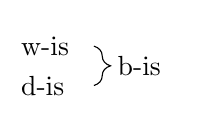
\begin{tikzpicture}[baseline]
			% Fixed coordinates
			\node (a1) at (-0,0) [text width=1.8cm, align=left] {\hspace*{-0.2cm}w-is};
			\node (a2) at (0,-0.5) [text width=1.8cm, align=left] {\hspace*{-0.2cm}d-is};
			
			% Curly brace from a1 to a2
			\draw[decorate,decoration={brace,amplitude=6pt}]
			([xshift=-1.2cm]a1.east) -- ([xshift=-1.2cm]a2.east);
			
			% Result node
			\node at (0.4,-0.25) {b-is};
		\end{tikzpicture} & \multirow{4}{*}{wit} \\
		& \cellcolor{gray!50} 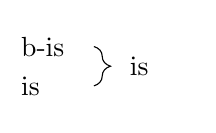
\begin{tikzpicture}[baseline]
			% Fixed coordinates
			\node (a1) at (-0,0) [text width=1.8cm, align=left] {\hspace*{-0.2cm}b-is};
			\node (a2) at (0,-0.5) [text width=1.8cm, align=left] {\hspace*{-0.2cm}is};
			
			% Curly brace from a1 to a2
			\draw[decorate,decoration={brace,amplitude=6pt}]
			([xshift=-1.2cm]a1.east) -- ([xshift=-1.2cm]a2.east);
			
			% Result node
			\node at (0.4,-0.25) {is};
		\end{tikzpicture} & \\
		\arrayrulecolor{white}
		\hline
		\textsc{dative} &
		\cellcolor{gray!50} 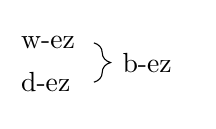
\begin{tikzpicture}[baseline]
			% Fixed coordinates
			\node (a1) at (0,0) [text width=1.8cm, align=left] {\hspace*{-0.2cm}w-ez};
			\node (a2) at (0,-0.5) [text width=1.8cm, align=left] {\hspace*{-0.2cm}d-ez};
			
			% Curly brace from a1 to a2
			\draw[decorate,decoration={brace,amplitude=6pt}]
			([xshift=-1.2cm]a1.east) -- ([xshift=-1.2cm]a2.east);
			
			% Result node
			\node at (0.5,-0.25) {b-ez};
		\end{tikzpicture} & \multirow{4}{*}{wa-s} \\
		& \cellcolor{gray!50} 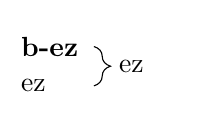
\begin{tikzpicture}[baseline]
			% Fixed coordinates
			\node (a1) at (-0,0) [text width=1.8cm, align=left] {\textbf{\hspace*{-0.2cm}b-ez}};
			\node (a2) at (0,-0.5) [text width=1.8cm, align=left] {\hspace*{-0.2cm}ez};
			
			% Curly brace from a1 to a2
			\draw[decorate,decoration={brace,amplitude=6pt}]
			([xshift=-1.2cm]a1.east) -- ([xshift=-1.2cm]a2.east);
			
			% Result node
			\node at (0.3,-0.25) {ez};
		\end{tikzpicture} & \\
		\arrayrulecolor{black}
		\textsc{comitative} & za-ɬːu & wa-ɬːu \\
		\textsc{similative} & za-qˤdi & wa-qˤdi \\
		\textsc{comparative} & za-χur & wa-χur \\
		\textsc{substitutive} & za-kɬ’ena & wa-kɬ’ena \\
		\textsc{superessive} & za-t & wa-t \\
		\textsc{superelative} & za-tːi-š & wa-tːi-š \\
		\textsc{superlative} & za-tːi-k & wa-tːi-k \\
		\textsc{superterminative} & za-tːi-kǝna & wa-tːi-kǝna \\
		\textsc{contelative} & za-ra-š & wa-ra-š \\
		\textsc{contlative} & za-ra-k & wa-ra-k \\
		\textsc{contallative} & za-r-ši & wa-r-ši \\
		\textsc{contterminative} & za-ra-kǝna & wa-ra-kǝna \\
		\lspbottomrule
	\end{tabularx}

	\begin{quote}
		Note: \\
		\textsc{‘cont’} in the names of spatial cases indicates contact location.
	\end{quote}
\end{table}

\begin{table}[p]
	\centering
	\renewcommand{\thetable}{9b}
	\caption{\ili{Archi} plural personal pronouns (partial paradigms), based on \citet[257--260]{kibrik1977} and \citet[102]{chumakinacorbett2015}}
	\label{01tab9b}
	\begin{tabularx}{0.85\textwidth}{llll}
		\lsptoprule
		\multicolumn{4}{c}{\textsc{plural}} \\
		\midrule
		& \multicolumn{2}{c}{\textsc{1 person}} & \textsc{2 person} \\
		& \textsc{exclusive} & \textsc{inclusive} & \\
		\midrule
		\textsc{absolutive} & \multirow{5}{*}{nen} & nen<t’>u & \multirow{5}{*}{žʷen} \\
		\arrayrulecolor{white}\cmidrule{3-3}
		\textsc{ergative} & & \cellcolor{gray!50}{nena<w>(u)} & \\
		& & \cellcolor{gray!50}{nena<r>u} & \\
		& & \cellcolor{gray!50}{nena<b>u} & \\
		& & \cellcolor{gray!50}{nen<t’>u etc.} & \\
		\arrayrulecolor{white}
		\hline
		\textsc{genitive} & \multicolumn{1}{l|}{\cellcolor{gray!50}{ulu}} & \cellcolor{gray!50}{la<w>u} & \multirow{4}{*}{wiš} \\
		& \multicolumn{1}{l|}{\cellcolor{gray!50}{d-olo}} & \cellcolor{gray!50}{la<r>u} & \\
		& \multicolumn{1}{l|}{\cellcolor{gray!50}{b-olo}} & \cellcolor{gray!50}{la<b>u} & \\
		& \multicolumn{1}{l|}{\cellcolor{gray!50}{olo etc.}} & \cellcolor{gray!50}{la<t’>u etc.} & \\
		\hline
		\textsc{dative} & \multicolumn{1}{l|}{\cellcolor{gray!50}{w-el}} & \cellcolor{gray!50}{w-ela<w>(u)} & \multirow{4}{*}{wež} \\
		& \multicolumn{1}{l|}{\cellcolor{gray!50}{d-el}} & \cellcolor{gray!50}{d-ela<r>u} & \\
		& \multicolumn{1}{l|}{\cellcolor{gray!50}{b-el}} & \cellcolor{gray!50}{b-ela<b>u} & \\
		&  \multicolumn{1}{l|}{\cellcolor{gray!50}{el etc.}} & \cellcolor{gray!50}{el<t’>u etc.} & \\
		\arrayrulecolor{black}
		\textsc{comitative} & la-ɬːu & & žʷa-ɬːu \\
		\textsc{similative} & la-qˤdi & & žʷa-qˤdi \\
		\textsc{comparative} & la-χur & & žʷa-χur \\
		\textsc{substitutive} & la-kɬ’ena & & žʷa-kɬ’ena \\
		\textsc{superessive} & la-t & & žʷa-t \\
		\textsc{superelative} & la-tːi-š & & žʷa-tːi-š \\
		\textsc{superlative} & la-tːi-k & & žʷa-tːi-k \\
		\textsc{superterminative} & la-tːi-kǝna & & žʷa-tːi-kǝna \\
		\textsc{contelative} & la-ra-š & & žʷa-ra-š \\
		\textsc{contlative} & la-ra-k & & žʷa-ra-k \\
		\textsc{contallative} & la-r-ši & & žʷa-r-ši \\
		\textsc{contterminative} & la-ra-kǝna & & žʷa-ra-kǝna \\
		\lspbottomrule
	\end{tabularx}

	\begin{quote}
		Note: ‘etc.’ in a cell indicates the pattern of \isi{syncretism} where the plural of \textsc{genders i} and \textsc{ii} matches \textsc{gender iii singular}, and the plural of \textsc{genders iii} and \textsc{iv} matches \textsc{gender iv singular}. \\
		\textsc{‘cont’} in the names of spatial cases indicates contact location.
	\end{quote}
\end{table}

% Reset numbering if you have other tables afterward
\addtocounter{table}{-1}
\renewcommand{\thetable}{\arabic{table}}

\largerpage
Each of the shaded cells in Tables \ref{01tab9a} and \ref{01tab9b} includes an additional paradigm comparable to Table \ref{01tab8}, with the same pattern of \isi{syncretism}. (For comparison with other languages of the family see \citealt[220--223]{kibrikkodzasov1990}.) This is precisely the situation which seemed unlikely. Its existence means that we have a full typology, as we shall see in Section \ref{01sec4.3}.

\subsection{The typology of partial inflectability} \label{01sec4.3}

Putting together the analyses in Section \ref{01sec4.1} and Section \ref{01sec4.2} we arrive at the \mbox{typology} shown in Table \ref{01fig2}.

\begin{table}[ht]
	\centering
	\captionsetup{width=\textwidth}
	\caption{Partial inflectability: Two dimensions of comparison: summary}
	\label{01fig2}
	\begin{tabularx}{\textwidth}{p{0.2cm}L{3.1cm}L{4.1cm}L{3.2cm}}
		\lsptoprule
		& & \multicolumn{2}{c}{definition of segments} \\
		\cmidrule{3-4}
		& & slab (featural) & cell(s) (morphomic) \\
		\cmidrule{3-4}
		\multirow{2}{*}{\rotatebox{90}{system}} & simple specification & Polish\il{Polish} \textit{muzeum} ‘museum’ & Russian\il{Russian} \textit{èxo} ‘echo’\\
		& multiple feature specification & {\ili{Mian} object \isi{agreement}} & {\ili{Archi} pronouns} \\
		\lspbottomrule
	\end{tabularx}
\end{table}

We see that our typology of partial inflectability is complete (Table \ref{01fig2}). This opens the way for future investigation of the distribution of examples over the four types. The degrees of inflectability found in each type also deserve further work: the examples found to date typically have fewer lexical items inflecting for the full featural possibilities than those which are partially uninflectable (see, for instance, Table \ref{01tab7} on \ili{Mian} verb types).

\section{Conditions (\textit{incoming} factors)} \label{01sec5}

In the canonical world, inflecting items realize their feature specifications fully, irrespective of external conditions. Thus a verb may have feature values for tense and aspect, and \isi{agreement} specifications, and this is sufficient to determine its form. That is, external conditions such as word order are irrelevant: a verb does not change its tense value when in clause-initial position, for instance. However, in the real world we do find significant instances where items inflect or do not inflect, subject to external conditions (in addition to the expected featural requirements imposed, for instance, by government and \isi{agreement}). Such conditions are non-canonical, since the syntax would be simpler without them. The result of such conditions has been termed ``constructional non-inflectedness''\is{constructional non-inflectedness|(} by \citet[144]{spencer2020}, and ``syntagmatic/contextual uninflectedness'' by \citet[14]{doleschal2000}. I first present the different types of conditions which lead to uninflectedness (full or partial), then in Section \ref{01sec5.5} I review the forms which result.

\subsection{Syntactic position: \ili{German}} \label{01sec5.1}

A classic example is provided by \ili{German} adjectives. In attributive position these inflect for case, number and gender, with two levels of reduced agreement\is{agreement!reduced} \citep[95--96]{corbett2006} to which I return in Section \ref{01sec5.5}. Elsewhere, notably in predicate position, adjectives are uninflected:

\begin{exe}
	\ex \label{01ex13}
	\gll Dies-er Artikel ist sehr interessant. \\
	this-\textsc{sg.m.nom} article\textsc{(m)[sg.nom]} be.\textsc{prs.3sg} very interesting \\
	\trans ‘This article is very interesting.’
\end{exe}

In (\ref{01ex13}) the adjective \textit{interessant} `interesting' lacks any inflection.\footnote{For the complex issue of the conditions on case marking and lack of inflection for case in \ili{German}, see \citet{spencer2009} and references there.} Hence the condition determining whether the adjective inflects is a syntactic one.

\subsection{Position in the phrase: Tsova-Tush\il{Tsova-Tush (\emph{also} Batsbi)}} \label{01sec5.2}

In several languages we find inflection restricted to the right edge of a nominal phrase (this may involve conjuncts or an attributive modifier and a noun). We might anticipate a simple external condition on inflection: the item on the right edge inflects, others do not. For instance, an attributive occurring phrase-finally would inflect, while if standing before a noun (hence not at the right edge), it would not. With this in mind, consider the data in Table \ref{01tab10}, from the Nakh language Tsova-Tush\il{Tsova-Tush (\emph{also} Batsbi)} (also known as Batsbi), as analysed by \citet{simswilliamsbaerman2021}.

\largerpage
\begin{table}[H]
	\centering
	\caption{Tsova-Tush\il{Tsova-Tush (\emph{also} Batsbi)} (bbl, \citealt[171--172]{holiskygagua1994}, \citealt[28]{simswilliamsbaerman2021})}
	\label{01tab10}
	\begin{tabularx}{0.9\textwidth}{lL{4cm}L{3.5cm}}
		\lsptoprule
			& Substantivized adjective in final position ‘bad one’ & Attributive adjective in phrase ‘bad child’ \\
			\midrule
			\textsc{absolutive} & mos:i\textsuperscript{n} & mos:i\textsuperscript{n} bader \\
			\textsc{ergative} & muis:čo-v & muis:čO	badre-v \\
			\textsc{genitive} & muis:čo-\textsuperscript{n} & muis:čO	badre-\textsuperscript{n} \\
			\textsc{dative} & muis:čo-n & muis:čO badre-n \\
		\lspbottomrule
	\end{tabularx}

\begin{quote}
	Note: \textsuperscript{n} indicates nasalization, O indicates a reduced vowel (word-final position).
\end{quote}
\end{table}

In Table \ref{01tab10} we see that the substantivized adjective in final position is indeed inflected; but when there is attributive adjective, followed by a noun, it is the noun which takes the inflection. Sims-William \& Baerman stress the word-order effect, given that group inflection is an area feature shared by various languages of the Caucasus. From this perspective, we have an external condition on the paradigm: inflection is found at the right edge of the nominal phrase (and note that the absolutive singular has the bare stem, a significative absence, Section \ref{01sec2.3}). However, this adjective is one that also has a stem alternation, contrasting absolutive and oblique (the remaining case values). Even when it does not bear the main inflection, it retains some inflection, that of the stem alternation.

\subsection{Featural condition: \ili{Sanskrit}} \label{01sec5.3}

I now turn to a different type of condition, found in the \ili{Sanskrit} (san) future, as presented by \citet{stump2013}. The tense in question, termed the periphrastic future,\footnote{See further \citet{lowe2017} for critical discussion of the periphrastic status of this future tense at different periods of \ili{Sanskrit} and for additional examples.} consists of a masculine agent noun and, in the first and second persons, a form of the copula; this is set out in Table \ref{01tab11}.

\begin{table}[ht]
	\centering
	\captionsetup{width=\textwidth}
	\caption{Periphrastic future-tense formation in \ili{Sanskrit} \citep[111]{stump2013}}
	\label{01tab11}
	\begin{tabularx}{\textwidth}{llXX}
		\lsptoprule
		\multicolumn{4}{c}{components} \\
		\midrule
		& & verb derivative & copula \\
		\midrule
		\multirow{8}{*}{\rotatebox{90}{\textsc{person}}} & 1 and 2 & agent-noun derivative & \textsc{present indicative active} \\
		& & \textsc{masculine} & (very rarely \textsc{middle}) forms of \\
		& & \textsc{nominative} & \textit{as} ‘be’ \\
		& & \textsc{singular} & \\
		& 3 & agent-noun derivative & [none] \\
		& & \textsc{masculine} & \\
		& & \textsc{nominative} & \\
		& & \textsc{singular / dual / plural} & \\
		\lspbottomrule
	\end{tabularx}
\end{table}

The forms of \textit{as} `be' are given in Table \ref{01tab12}. This verb has all forms available, though the third person forms do not appear in the periphrastic tense in question.

\begin{table}[ht]
	\centering
	\captionsetup{width=\textwidth}
	\caption{Present indicative active of \textit{as} ‘be’ in \ili{Sanskrit} \citep[111]{stump2013}}
	\label{01tab12}
	\begin{tabularx}{0.6\textwidth}{XXXX}
		\lsptoprule
			& \textsc{singular} & \textsc{dual} & \textsc{plural} \\
			\midrule
			1 & ásmi & svás & smás \\
			2 & ási & sthás & sthá \\
			3 & ásti & stás & sánti \\
		\lspbottomrule
	\end{tabularx}
\end{table}

More importantly, for our purposes, the agent noun also has a full paradigm, distinguishing number, gender and case. With that in mind, consider the paradigm in Table \ref{01tab13}.

\begin{table}[ht]
	\centering
	\caption{Periphrastic future-tense forms of \textit{dā} ‘give’, without sandhi \citep[111]{stump2013}}
	\label{01tab13}
	\begin{tabularx}{0.7\textwidth}{XXXX}
		\lsptoprule
		& \textsc{singular} & \textsc{dual} & \textsc{plural} \\
		\midrule
		1 & dātā́ asmi & dātā́ svas & dātā́ smas \\
		2 & dātā́ asi & dātā́ sthas & dātā́ stha \\
		3 & dātā́ & {\charis\small \textbf{dātā́rau}} & {\charis\small \textbf{dātā́ras}} \\
		\lspbottomrule
	\end{tabularx}
\end{table}

Presenting the paradigm in this form is helpful, since it shows the partial inflectability which interests us. Of the full paradigm of the agent nominal, we find just the number distinction, and that only for third person forms. This can be seen, though less obviously, in the ``surface'' forms, those which arise as a result of automatic sandhi processes, where the two parts are pronounced as a single phonological word (see Table \ref{01tab14}). In the examples, sandhi is indicated by {\charis ‿}.

\begin{table}[ht]
	\centering
	\caption{Periphrastic future-tense forms of \textit{dā} ‘give’, with sandhi \citep[111]{stump2013}}
	\label{01tab14}
	\begin{tabularx}{0.6\textwidth}{XXXX}
		\lsptoprule
		& \textsc{singular} & \textsc{dual} & \textsc{plural} \\
		\midrule
		1 & dātā́smi & dātā́svas & dātā́smas \\
		2 & dātā́si & dātā́sthas & dātā́stha \\
		3 & dātā́ & {\charis\small \textbf{dātā́rau}} & {\charis\small \textbf{dātā́ras}} \\
		\lspbottomrule
	\end{tabularx}
\end{table}

\largerpage[2]
The key point for our analysis is that the agent nominal has a full paradigm, but when used in this future tense it inflects partially: it does not inflect when the periphrastic verb is first or second person; for the third person the agent nominal inflects for number but not for gender (only the masculine is found).\footnote{We see distributed exponence here: where the agent nominal is uninflectable for number, the auxiliary is present, and inflects for number; when the auxiliary is absent (in the third person) the agent nominal marks number.} Let us see how this works in examples:

\begin{exe}
	\ex \ili{Sanskrit} \citep[112]{stump2013} \label{01ex14} \\
	\gll Tatas tvā pārayitā{\charis ‿}asmi. \\
	from.that	\textsc{2sg.acc} 	rescue.\textsc{nmlz.sg.m}{\charis ‿}be.\textsc{prs.1sg} \\
	\trans ‘I will rescue (lit: I am rescuer) you from that.’ \\
	\hfill (\textit{Śatapatha Brāhmaṇa} 1.8.1.2)
\end{exe}

In (\ref{01ex14}) we have a first person singular subject, and the agent nominal is masculine singular. There is also a direct object (\textit{tvā} `you'), in the accusative, showing that this tense is not an ordinary predicate nominal construction. Compare the plural in (\ref{01ex15}):

\begin{exe}
	\ex \ili{Sanskrit} (part of example in \citealt[113]{stump2013}) \label{01ex15} \\
	\gll Mahac	{\charis ‿}choka-bhayam	prāptā{\charis ‿}smaḥ.\footnotemark \\
	great.\textsc{sg.acc}	pain-fear.\textsc{sg.acc}	meet.\textsc{nmlz.sg.m}{\charis ‿}be.\textsc{prs.1pl} \\
	\trans ‘We are going to meet with great pain and dread.’ \\
	\hfill (\textit{Gopatha Brāhmaṇa} 1.1.28)
	
	\footnotetext{\textit{smaḥ} is the pre-pausal sandhi variant of the first person plural \textit{smas} (Greg Stump, personal communication, 5 August 2013).}
\end{exe}

Note that although we have a plural subject, the agent nominal remains singular here (since the verb is first person). I now move to the third person:

\begin{exe}
	\ex \ili{Sanskrit} \citep[113]{stump2013} \label{01ex16} \\
	\gll Ekā jananayitā putram. \\
	one.\textsc{sg.nom.f}	produce.\textsc{nmlz.sg.m}	son.\textsc{sg.acc} \\
	\trans ‘One (feminine) will bear a son.’ \hfill (\textit{Rāmāyaṇa} 1.38.8)
\end{exe}

Example (\ref{01ex16}) is significant: the subject is third person (so no copula); it is clearly feminine, but the agent nominal maintains masculine gender. However, the agent nominal can inflect (for number) in future tense use, as example (\ref{01ex17}) shows:

\begin{exe}
	\ex \ili{Sanskrit} \citep[114]{stump2013} \label{01ex17} \\
	\gll Na	jāne	yātāras	tava	ripavaḥ	kena	ca	pathā. \\
	not	know.\textsc{1sg}	go.\textsc{nmlz.pl.m}	thy	enemy.\textsc{pl.nom}	which.\textsc{sg.ins}	and	path.\textsc{sg.ins} \\
	\trans ‘I don’t know by which path your enemies will go.’ \hfill (\textit{Bhojaprabandha} 55)
\end{exe}

Here we see a third plural subject and the agent nominal is plural. This fits with the pattern in Table \ref{01tab11}. The agent nominal has a full paradigm, but when used for the future it does not inflect at all when the subject is first or second person; when the subject is third person it inflects for number (\ref{01ex17}) but not gender (\ref{01ex16}). The agent nominal's pattern of partial inflection is conditioned by the person of the subject, that is, by a featural specification.

\subsection{Further instances} \label{01sec5.4}

Other examples of external conditions include the following varied selection. Proper names may be accompanied by classifier-like nouns (sortals) and the proper name may then remain uninflected. See \citet{matushansky2022, matushansky2023} for careful discussion of these constructions in \ili{Russian}. An example is given in (\ref{01ex18}):

\begin{exe}
	\ex \ili{Russian} \citep[235]{matushansky2023} \label{01ex18} \\
	\gll na	ulic-e / *ulic-a \phantom{xxxxxxxxxxxxxxxxxx} Jakimank-e / Jakimank-a \\
	on	street-\textsc{sg.loc} / *street-\textsc{sg.nom} \phantom{xxxxxxxxxxxxxxxxxx} Yakimanka-\textsc{sg.loc} / Yakimanka-\textsc{sg.nom}  \\
	\trans ‘on Yakimanka Street’
\end{exe}

In this instance (see \citealt{matushansky2023} for the other types), while the sortal noun must take the case value required by the syntactic context, the proper name may be in that case or may stand in the nominative. For appositives in \ili{Polish} see \citet{cetnarowska2021}.

In \ili{Kayardild}, the external condition is that the set of words on which a morphosyntactic feature is realized is determined by concentric domains of features \citep[78--84]{round2013}. In \ili{Lithuanian} \citet{arkadiev2013, arkadiev2020}, participles agree or lack \isi{agreement} morphology depending on the construction (and there is a complex web of interrelated constructions). \citet{giger2016} describes the loss of inflection of participles as a participial perfect emerges in \ili{Slovak}. And for the interesting complexities of \ili{Hungarian} inflecting infinitives and \ili{Latvian} genitive compounds see \citeauthor{spencer2025} (this volume).

\subsection{Forms used and distinctions retained in constructional non-inflectedness} \label{01sec5.5}

I have so far examined the types of construction which condition (often partial) non-inflectedness. I now switch my focus to the forms used in examples of constructional non‑inflectedness, and the distinctions retained. The clearest type is that found in the \ili{German} predicate adjective (example (\ref{01ex13})); this takes a form lacking all inflection, and retaining none of the featural distinctions of inflected forms. This implies two distinctions. First, there are uniquely uninflected forms, as in our \ili{German} example, opposed to normal inflected forms, used for constructional non‑inflectedness, such as the \ili{Russian} nominative (Section \ref{01sec5.4}). Second, there are forms where no distinctions are retained, as in the \ili{German} example, opposed to those where at least one distinction is retained, as in Tsova-Tush\il{Tsova-Tush (\emph{also} Batsbi)}. Significant examples are given in Table \ref{01tab15}, and then key points are highlighted.

\begin{table}[ht]
	\centering
	\caption{Forms and distinctions in constructional non‑inflectedness\is{constructional non-inflectedness|)}}
	\label{01tab15}
	\begin{tabularx}{\textwidth}{>{\raggedright}p{3.7cm}QQQ}%L{3.7cm}L{2.5cm}L{2.2cm}L{2.5cm}
		\lsptoprule
			example & unique vs normal forms & featural distinctions retained & source \\
			\midrule
			German\il{German} predicative adjective & unique & none & see Section \ref{01sec5.1} \\
			Tsova-Tush\il{Tsova-Tush (\emph{also} Batsbi)} attributive adjective (not phrase-final) & unique & \textsc{absolutive} vs \textsc{oblique} & see Section \ref{01sec5.2} \\
			Somali\il{Somali} verb (subject focus) & unique & \textsc{3sg.f} / \textsc{1pl} / rest & \citet[93, 203--204]{corbett2006} and references there  \\
			Inari Saami\il{Inari Saami} reduced agreement\is{agreement!reduced} & normal & \textsc{sg} vs \textsc{du-pl} & \citet[94--95]{corbett2006}, \citet{toivonen2007} \\
			Russian\il{Russian} sortal noun & normal: \textsc{nominative} & \textsc{sg} vs \textsc{pl} & see Section \ref{01sec5.4} \\
			Sanskrit\il{Sanskrit} periphrastic future & normal: \textsc{masculine} (and \textsc{singular} in person 1 and 2) & \textsc{sg} vs \textsc{du} vs \textsc{pl} (in person 3) & see Section \ref{01sec5.3}, \citet{stump2013} \\
			German\il{German} attributive adjective & normal & \textsc{case} and \textsc{number} (limited degree) & \citet[95--96]{corbett2006} \\
		\lspbottomrule
	\end{tabularx}
\end{table}

\largerpage
\ili{Somali} deserves mention since it has reduced agreement\is{agreement!reduced} forms which are unique to the reduced paradigm; furthermore, the distinctions made in the reduced paradigm are not a simple collapsing on those in the full paradigm (as in Tsova-Tush\il{Tsova-Tush (\emph{also} Batsbi)}), but rather the patterns of \isi{syncretism} are different. \ili{Inari Saami} is included because the reduced paradigm has no unique forms; it retains the third person singular and the third plural from the full paradigm, and these fill out the reduced paradigm. Reduced agreement\is{agreement!reduced} (\citealt{feddenpaciaroni2022}, and \citeauthor{loporcaro2025}, this volume), a subset of partial inflection determined by external conditions, is a fruitful area to work on, because \isi{agreement} allows us to manipulate the feature values involved, which can be useful for establishing the nature of the partially inflected forms. Continuing with the data in Table \ref{01tab15}, the \ili{Sanskrit} periphrastic future (Section \ref{01sec5.3}) is illuminating because we find possible inflected forms, but used beyond their normal range. Here we can ask whether we have a default form (an inflected form used when there is no specification). This is a plausible analysis for the \ili{Sanskrit} future, where we find masculine as the gender default, and singular as the number default. (The nominative is expected as the case value in the predicate.) However, in the third person, distinctions of number are retained: we have a reduced paradigm rather than a single default form. Thus the features in \ili{Sanskrit} have sufficient values for it to be clear what is going on; we need to beware of small systems, which can be misleading.\footnote{There is careful discussion of default \isi{agreement} vs lack of \isi{agreement} inflection in \ili{Lithuanian} in \citet[383--387, 403-404, 408-412]{arkadiev2020}. And one needs to establish the default instance by instance; thus in \ili{Serbo-Croat} \citep[329, 374]{browne1993-serbocroat} and \ili{Polish} the accusative is an attractor for length-of-time and quantity constructions.} Finally, we need to note the complexities of \ili{German} adjectives in attributive position. There are two stages of reduction: the paradigms are traditionally labelled strong, mixed and weak. There is a notional paradigm with 16 cells (four case values, plural vs singular and -- in the singular -- three gender values). However, there are extensive syncretisms\is{syncretism} so that even the strong paradigm has only five distinct forms. The mixed paradigm has four of those forms, and the weak has only two; however, we do not find a straightforward collapsing of distinctions, but rather we see different patterns of \isi{syncretism}. The mixed and weak paradigms retain some distinction within each of the features (case, number and person).

\largerpage
We have observed that there are lexemes which do not inflect, even though this might be expected (Section \ref{01sec3}), and this uninflectability is a matter of degree (Section \ref{01sec4}). In this section (Section \ref{01sec5}), we have seen that there are external conditions which determine whether otherwise inflecting items inflect. And here too it is a matter of degree. I now turn to the final logical possibility, the possible outward effect of uninflectability.

\section{External consequences (\textit{outgoing})} \label{01sec6}

Since uninflectability is a matter of inflection, one would expect no syntactic consequences. We do find instances of this canonical situation (Section \ref{01sec6.1}), but there are also claims in the literature that uninflectability has consequences, and I discuss some of these (Section \ref{01sec6.2}).

\subsection{No external consequences} \label{01sec6.1}

Often this situation is simply assumed: researchers report the inflectional situation and imply that there is no more to be said. However, there are also studies which look carefully for external consequences, and do not find any. I consider in turn \citet{nichols2018} on \ili{Ingush}, and \citet{fedden2022} on \ili{Mian}.

\subsubsection{Agreement\is{agreement} in \ili{Ingush} (Nakh-Dagestanian)} \label{01sec6.1.1}

\ili{Ingush} (inh), which has some 300,000 speakers living mainly in Ingushetia in the North Caucasus, is a Nakh language (hence a relative of Tsova-Tush\il{Tsova-Tush (\emph{also} Batsbi)}, discussed in Section \ref{01sec5.2} and a more distant relative of \ili{Archi}, introduced in Section \ref{01sec1.3} and Section \ref{01sec3.1.2}). It has ``an arbitrary\is{arbitrary vs. motivated} and strictly lexical bifurcation of verbs'' \citep[845]{nichols2018}, in that some have gender and number \isi{agreement} and some do not. There are 400 simple verbs at most, of which around 30\% show gender and number \isi{agreement} (change of the initial consonant); however, there are other possibilities, including light verbs and tense auxiliaries, so that inflected verb forms have some gender and number \isi{agreement} in probably well over 50\% of the instances \citep[141n63, 235]{nichols2011}.\footnote{That is 90/294 (30.6\%) of the simple verb roots; if those with number distinctions (verbal number) are included, the figure is 109/393 (27.7\%). Of the simple adjectives, fewer than 10\% take \isi{agreement} \citep[141]{nichols2011}. See \citet[141--145]{nichols2011} for details on the relation of gender and number in \isi{agreement}.} Given this situation, we can use variation in one phenomenon (inflection for \isi{agreement} or lack of it) to test proposed explanations for another. Thus it is sometimes suggested that the function of \isi{agreement} is to facilitate reference tracking. By comparing agreeing with non-agreeing verbs, one can ask whether we can see differences in other means of reference tracking, in particular the presence of an overt argument (which might be introduced to facilitate reference tracking when the verb does not agree). \citet{nichols2018} has measured carefully, using a corpus of narrative texts (mainly spoken). The results are summarized in Table \ref{01tab16}.

\begin{table}[ht]
	\centering
	\caption{\ili{Ingush}: verb \isi{agreement} and overt arguments (tokens) (from \citealt[858]{nichols2018})}
	\label{01tab16}
	\begin{tabularx}{0.95\textwidth}{llrrrr}
		\lsptoprule
			& & \textsc{s} & \textsc{a} & \textsc{o/t} & total \\
			\midrule
			\multirow{2}{*}{verb root agrees} & n & 100 & 41 & 37 & 178 \\
			& \% overt argument & 88 & 59 &	92 & \cellcolor{gray!25}82 \\
			\midrule
			\multirow{2}{*}{verb root does not agree} & n & 41 & 38 & 24 & 103 \\
			& \% overt argument & 85 & 76 &	83 & \cellcolor{gray!25}82 \\			
		\lspbottomrule
	\end{tabularx}

\begin{quote}
	Note: \\
	\textsc{s}: single argument of intransitive verb; \textsc{a}: agent-like argument of a monotransitive; \textsc{o}: direct object of a monotransitive; \textsc{t}: theme-like or patient-like object of a ditransitive
\end{quote}
\vspace*{-0.7cm}
\end{table}

We see that there is no difference between the examples with an agreeing verb and those with a non-agreeing verb. The morphological difference is not reflected in the syntax. For comparable results from the Dagestanian language Lak, see \citet{forker2018}.

\subsubsection{Agreement\is{agreement} in \ili{Mian}} \label{01sec6.1.2}

\ili{Mian} was introduced in Section \ref{01sec4.2}. Based on a fully annotated \ili{Mian} test corpus of 14 texts, some 4,000 words, with around 1,700 clauses, \citet{fedden2022} undertook a study similar to that of \citet{nichols2018}, discussed in Section \ref{01sec6.1.1}. Here we are concerned only with object \isi{agreement}, since all verbs show subject \isi{agreement}. There are three types of transitive verb; recall from Table \ref{01tab7} that only 16\% of \ili{Mian} verbs show object \isi{agreement}, 2\% showing \isi{agreement} in person, number and gender and 14\% taking gender 2. Thus object \isi{agreement} is relevant for a lower proportion of the transitive verbs than that found in \ili{Ingush}. Due to the high type and token frequency of non-agreeing verbs, the syntax is constantly encountering gaps. What then can we learn about reference tracking? The data on the presence of overt arguments are given in Table \ref{01tab17}.

\begin{table}[ht]
	\centering
	\caption{\ili{Mian} object \isi{agreement}: verb agrees or not \citep[300]{fedden2022}}
	\label{01tab17}
	\begin{tabularx}{0.85\textwidth}{llrrr}
		\lsptoprule
		& & gender & gender 2 & combined \\
		\midrule
		\multirow{2}{*}{verb agrees} & n & 61 & 218 & 279 \\
		& \% overt & 33 & 39 & \cellcolor{gray!25}38 \\
		\midrule
		\multirow{2}{*}{verb does not agree} & n & & & 397 \\
		& \% overt & & & \cellcolor{gray!25}43 \\			
		\lspbottomrule
	\end{tabularx}
\end{table}

The difference between the highlighted cells is not statistically significant. And so, although the situation in \ili{Mian} is rather different from that in \ili{Ingush}, we find again that inflectability has no syntactic effect.

\subsection{External (syntactic) consequences} \label{01sec6.2}

There are various places in the literature where it is claimed that uninflectability does have syntactic consequences. I will report the data on some of the suggested examples (I have carried out only limited fieldwork and cannot vouch for them). I will note the others briefly. Typically there is speaker variation.

\subsubsection{\ili{Serbo-Croat} \textit{doba} `time, season, age, period'} \label{01sec6.2.1}

This noun is unusual in several ways, including the fact that it is the only neuter noun in the language with the nominative singular in \textit{-a}. In a language where uninflectability is rare (\citealt[378]{browne1993-serbocroat}; \citealt{browne1993-nps}), this noun is often cited in grammars and dictionaries as uninflectable, with \textit{doba} as its unique form. However, the situation is more complex, as was pointed out as early as \citet[246]{kovacevic1951}, see also \citet[212--214]{stevanovic1975} and \citet[16--17]{nikolic1995-96}. The potential paradigm is given in Table \ref{01tab18}, though the use of the form \textit{doba} is found in other cells of the paradigm too.

\begin{table}[ht]
	\centering
	\caption{Inflection of \ili{Serbo-Croat} \textit{doba} ‘time’ \citep[79]{benson1971}}
	\label{01tab18}
	\begin{tabularx}{0.6\textwidth}{lXX}
		\lsptoprule
		& \textsc{singular} & \textsc{plural} \\
		\midrule
		\textsc{nominative} & doba & doba \\
		\textsc{accusative} & doba & doba \\
		\textsc{genitive} & doba & dobā \\
		\textsc{dative} & dobu & dobima \\
		\textsc{locative} & dobu & dobima \\
		\textsc{instrumental} & dobom & dobima \\
		\lspbottomrule
	\end{tabularx}
\end{table}

Our concern here is those instances when the noun remains uninflectable, since attributive modifiers can be affected by the uninflectability of the noun. There are examples in both \citet{kovacevic1951} and \citet{stevanovic1975} of phrases with \textit{doba} `time', governed by a preposition, where the attributive modifier appears to follow the form of \textit{doba} rather than standing in the appropriate case. Consider these alternatives:

\begin{exe}
% 	\needspace{6\baselineskip}
	\ex  \ili{Serbo-Croat} (\citealt{kovacevic1951} and web sources) \vspace*{-0.3cm}
	\begin{multicols}{2}
	\begin{xlist}
		\ex \label{01ex19a}
		\gll u	t-om	doba \\
		in	that-\textsc{sg.loc.n/m} time \\
		\trans ‘at that time’
		\ex \label{01ex19b}
		\gll u	t-o	doba \\
		in	that-\textsc{sg.acc.n}	time \\
		\trans ‘at that time’
	\end{xlist}
	\end{multicols}
\end{exe}

The use of the locative modifier with the uninflected \textit{doba} is rare (\ref{01ex19a}); much more common is the use of the \textit{to} form of the demonstrative (\ref{01ex19b}). We can treat this as the accusative, and note two factors here. First the accusative tends to be used, rather than the locative, more generally in such time expressions: this is true both for other attributive modifiers of \textit{doba} `time' \citep[11--13]{browne2015} and for other nouns denoting time which do not have the unusual characteristics of \textit{doba}. And second, \textit{to doba} `that time' could be analysed as moving towards being an adverbial expression, a fixed phrase unaffected by external government. We therefore take a preposition governing the genitive case: then the first factor no longer applies, while the second does. \citet{browne2015} reports a web count of three relevant examples:

\vspace{0.4cm}

\noindent \citet[12]{browne2015}: web count 31.12.2014
\begin{exe}
	\ex \label{01ex20}
	\gll od t-og doba \hspace{2.8cm} 285 instances: 43.5\% \\
	from that-\textsc{sg.gen.n/m} time \\
	\trans ‘from that time’
	
	\ex \label{01ex21}
	\gll od t-oga doba \hspace{2cm} 242 instances: 36.9\% \\
	from that-long.\textsc{sg.gen.n/m} time \\
	\trans ‘from that time’
	
	\ex \label{01ex22}
	\gll od t-o doba \hspace{2.4cm} 128 instances: 19.5\% \\
	from that-\textsc{sg.nom/acc.n} time \\
	\trans ‘from that time’
\end{exe}

Since \textit{od} `from' takes the genitive, (\ref{01ex20}) and (\ref{01ex21}) are as expected. But a minority of instances as in (\ref{01ex22}) show that \textit{doba} `time' does not always behave as we would expect from an uninflectable noun. Rather we find a syncretic nominative-accusative form, which we take as accusative for the reasons given above. But this would imply that we have different behaviours, depending on the particular cell of the paradigm (Section \ref{01sec4.1}). Given that, the suggestion that \textit{to doba} `that time' is becoming a fixed adverbial expression of time, impervious to case government, seems a reasonable one.

\subsubsection{\ili{Serbo-Croat} numeral phrases\is{numeral phrase|(}} \label{01sec6.2.2}

\ili{Serbo-Croat} numerals have largely lost inflection. The higher numerals, \textit{pet} `five' and above, typically do not inflect (and they take the genitive plural of the quantified noun).\footnote{They lost inflection in the 16\textsuperscript{th} to 17\textsuperscript{th} centuries, according to \citet[138]{rogic1954}. However, the higher, more noun-like numerals (\textit{stotina} `hundred', \textit{tisuća} and \textit{hiljad} `thousand', \textit{milion} and \textit{milijun} `million') can inflect, particularly in complex numerals, or stand in the accusative \citep[11--12]{popovic1979}.} The numerals \textit{dva} `two' (masculine and neuter, with \textit{dve} feminine), \textit{tri} `three' and \textit{četiri} `four' are losing inflection for case, but have not done so completely, and this has engendered a substantial literature.\footnote{\citet{markovic1951} pointed out that \textit{dva} `two', and even more so, \textit{tri} `three' and \textit{četiri} `four' were becoming uninflectable for case; this change was well under way in the 19\textsuperscript{th} century, and he discusses instances where inflection is preserved in relevant texts. He noted already the tendency for numeral phrases which would be in the instrumental to be replaced with \textit{s} `with' and the uninflectable form of the numeral. \citet{rogic1954} gives examples illustrating the loss of inflection of these numerals. \citet{hamm1956} discusses grammarians' statements on the topic and usage in the press. M. \citet{popovic1967} talks of ``blocks'' which inflect, meaning that in constructions consisting of preposition + numeral + noun, the numeral and noun form a `block' whose case is registered in the preposition. The journal \textit{Naš jezik} had three papers on the topic in 1976: \citet{kraljevic1976} gives a wealth of data, including dialect data, showing that lack of inflection is more prevalent in the east; \citet{nikolic1976} gives summary information on 28 dialects, showing that inflection of the numeral is more likely if the noun is feminine, more likely in the dative, locative and instrumental cases than in the genitive, more likely with \textit{dva} `two' than with \textit{tri} `three', and more likely with \textit{tri} `three' than with \textit{četiri} `four'; \citet{radovictesic1976} concentrates on the range of forms of the numerals. Lj. \citet{popovic1979} discusses uninflectability within the general morphosyntactic system of the numerals; his papers on uninflectability and the dative are discussed in the main text. \citet{durovic1985} also gives a general account, including uninflectedness, as does \citet{browne2022}, while \citet{grubisic1994} discusses the grammatical tradition on the topic. \citet{kuzmic2007} examines Čakavian legal texts (13\textsuperscript{th}--18\textsuperscript{th} centuries) while \citet{kuzmickuzmic2007} analyse Kajkavian legal texts (16\textsuperscript{th}--18\textsuperscript{th} centuries); both papers provide a wealth of textual examples from the respective varieties, including evidence on the rise of uninflectability. \citet[148--193]{stefanovic2019} provides many examples, of both inflectedness and uninflectedness.} These lower numerals require the \textit{\isi{adnumerative}} of the quantified noun, and this is realized as the genitive singular or the nominative plural, depending on the inflection class of the noun \citep[159--160]{corbett2009}. For our purposes, the typical situation is the interesting one, that where numeral phrases increasingly function as non-inflecting units; that is, the numeral does not inflect, and it determines the inflectional form of the quantified noun, giving a constituent which is impervious to external syntax. In other words, a numeral + noun unit (given in square brackets in our examples) behaves somewhat like an uninflectable noun. Such phrases are fine when they occur in syntactic positions requiring the nominative, accusative or genitive case; the latter is illustrated in (\ref{01ex23}):

\begin{exe}
	\ex \ili{Serbo-Croat} \citep[150]{wechslerzlatic2003} \label{01ex23} \\
	\gll Seć-am	se	[ova četiri glumca].\footnotemark \hspace{2cm} [\textsc{genitive}] \\
	remember-\textsc{prs.1sg} \textsc{refl} \textsc{dem} four actor \\
	\trans ‘I remember these four actors.’
\end{exe}

\footnotetext{Here \textit{glumca} ‘actor’ is in the \isi{adnumerative}, realized as the genitive singular; \textit{ova} ‘these’ is also in the \isi{adnumerative}, realized as the nominative plural neuter \citep[17--18]{corbett2023}.}

They are also fully acceptable with prepositions taking various cases, as in (\ref{01ex24}):

\begin{exe}
	\ex \ili{Serbo-Croat} \citep[150]{wechslerzlatic2003} \label{01ex24} \\
	\gll Razgovar-am 	sa	[ova četiri glumca]. \hspace{1.5cm} [\textit{sa} + \textsc{instrumental}] \\
	talk-\textsc{prs.1sg}	with	\textsc{dem} four actor \\
	\trans ‘I am talking to these four actors.’
\end{exe}

However, these numeral phrases do not fit everywhere. As pointed out by Lj. \citeauthor{popovic1981-1982} (\citeyear{popovic1981-1982}, see also \citeyear{popovic1982}), the case frame matters: they do not work as a dative:\footnote{I give examples from the extended discussion by Wechsler \& Zlatić, since they are simpler than those in the original. See also \citet[374--375]{browne1993-serbocroat}. As for the remaining two case values: (i) the locative is found only with prepositions, and so it causes no problem; (ii) the instrumental, interestingly, can be replaced in these constructions by \textit{sa} `with' plus the uninflected unit, to give an acceptable form comparable to (\ref{01ex24}). There is no comparable escape for the dative (Lj. \citealt[606]{popovic1981-1982}).}

\begin{exe}
	\ex \ili{Serbo-Croat} \citep[150]{wechslerzlatic2003} \label{01ex25} \\
	\gll *dati	knjig-e	[ova četiri studenta] \hspace{2.6cm} [*\textsc{dative}] \\
	give.\textsc{inf}	book\textsc{-pl.acc}	\textsc{dem} four student \\
	\trans ‘to give books to these four students’
\end{exe}

This is indeed surprising; in some case frames the lack of morphological realization of the case value is unproblematic, while for the dative there is an issue (\ref{01ex25}). The non-inflecting unit behaves as though it is defective\is{defectiveness}, lacking a dative case form. There is further discussion in \citet[148--152]{wechslerzlatic2003}, \citet{franks2024} and for higher numerals in \citet{boskovic2006}.

I have concentrated on numeral phrases; according to \citep[133--140]{wechslerzlatic2003} similar issues of inflectability depending on the case value arise with uninflectable \textit{nouns} in \ili{Serbo-Croat}. (There are relatively few of these, but female names such as \textit{Dolôres}, which do not match the appropriate \ili{Serbo-Croat} inflectional pattern, are uninflectable, as noted in Section \ref{01sec3.2}.) \citet[107n3]{ivic1972} pointed out that their use in an oblique case is facilitated by the presence of a modifier or a preposition. See also \citet{boskovic2006, boskovic2009}; \citet{horvath2014} and \citet[103--111]{adamson2019} on this; there is speaker variation here. External effects have also been suggested for uninflectable \textit{adjectives}; \ili{Serbo-Croat} also has some instances, many of them orientalisms, as documented in \citet{nikolic1996}. \citet[22]{boskovic2013} claims that these have syntactic effects, notably that an uninflectable adjective must be adjacent to its head noun. His account is discussed in \citet[115--121]{adamson2019}. There is speaker variation here too.\footnote{\citet[121--131]{adamson2019} discusses \ili{Italian} uninflectable adjectives, and concludes that their inability to appear in prenominal position, when unmodified, is not a direct result of their lack of inflection. Hence this is not a case for inclusion here.} \citet[160--184]{adamson2019} further analyses \ili{German} prenominal uninflectable adjectives and argues that here there is a syntactic effect in that they do not allow noun phrase ellipsis\is{numeral phrase|)}.

\subsubsection{Definiteness\is{definiteness} in \ili{Bulgarian}}

The relevance of \isi{definiteness} in \ili{Bulgarian} was first pointed out by \citet[150--153]{halpern1995}; see also \citet[128--130]{spencerluis2012}; it is of ongoing interest, as shown by \citeauthor{adamson2019} (\citeyear[83--103]{adamson2019}; \citeyear{adamson2022}) and \citet{georgieva2023}. In \ili{Bulgarian}, \isi{definiteness} is inflectional, and a nominal phrase can be marked definite on the first markable item:\footnote{I thank Vladimir Zhobov for his help with the \ili{Bulgarian} data.}

\vspace*{0.3cm}

%\needspace{4\baselineskip}
\noindent \ili{Bulgarian} (bul, \citealt[128--130]{spencerluis2012})
\begin{exe}
	\ex  \label{01ex26}
	\gll knig-a-ta \\
	book\textsc{(f)-sg-def.sg.f} \\
	\trans ‘the book’
	
	\ex  \label{01ex27}
	\gll xubav-a-ta		knig-a \\
	nice-\textsc{sg.f-def.sg.f}	book\textsc{(f)-sg}  \\
	\trans ‘the nice book’
\end{exe}

Example (\ref{01ex26}) shows \isi{definiteness} marking on the noun since it is the only item in the phrase, while in (\ref{01ex27}) it is on the adjective, as the first markable item. The issue arises where we have an item like \textit{serbez} `quarrelsome', which the cited researchers analyse as an uninflectable adjective. When the phrase is indefinite, all is well, as in (\ref{01ex28}):

\begin{exe}
	\ex \ili{Bulgarian} (\citealt[150--153]{halpern1995}, \citealt[128--130]{spencerluis2012}) \label{01ex28} \\
	\gll serbez		žen-a \\
	quarrelsome	woman\textsc{(f)-sg} \\
	\trans ‘a quarrelsome woman’
\end{exe}

The issue arises when the phrase is definite. If \textit{serbez} `quarrelsome' counts as the first element (as we would expect given (\ref{01ex27})), ungrammaticality results (the alternatives show the ways that \isi{definiteness} might, theoretically, be shown on it):

\begin{exe}
	\ex \label{01ex29}
	\gll *serbez-ăt/ta		žen-a \\
	quarrelsome-\textsc{def.sg} 	woman\textsc{(f)-sg} \\
	\trans ‘the quarrelsome woman’
\end{exe}

Clearly, then, \textit{serbez} `quarrelsome' does not count as the first element for \isi{definiteness}. But if it is not counted, the result is also ungrammatical:

\begin{exe}
	\ex \label{01ex30}
	\gll *serbez	žen-a-ta\footnotemark \\
	quarrelsome	woman\textsc{(f)-sg-def.sg.f} \\
	\trans ‘the quarrelsome woman’
\end{exe}

\footnotetext{\citeauthor{halpern1995} states (\citeyear[165n22]{halpern1995}) that this example is possible as an ‘‘ironic or humorous quotation’’ of a previous description.}

Thus neither way works: uninflectable \textit{serbez} `quarrelsome' neither accepts \isi{definiteness} marking nor allows it on the noun; it neither counts as the first element nor allows the noun to be the first element. Hence we do appear to have an instance where uninflectability has an external effect on the syntax.

\subsection{External (syntactic) consequences: summing up}

I have presented three possible instances and noted others; South Slavonic is well represented. Each case is challenging, and there is speaker variation to be reckoned with. In this section, the key issue is not whether the item inflects, but how similar it is syntactically to regular inflecting items. The \ili{Serbo-Croat} numeral phrases (Section \ref{01sec6.2.2}) are significant, since they show \isi{defectiveness}, in that they fail to fit into syntactic slots where a dative would be required.\footnote{\citet{testelets2010} offers interesting discussion of case deficiency more generally, based on \ili{Russian} data.}

\section{Conclusions} \label{01sec7}

I have explored the logical space of uninflectability. First, I calibrated uninflectability across items, determining which items have the property, and how they can be specified. Second, I determined the extent of uninflectability within items. Third, I noted the possible \textit{incoming} conditions on uninflectability. And fourth, I evaluated the \textit{outgoing} requirements imposed by uninflectable items.

What then can we learn when the dog doesn't bark, when an item doesn't inflect? This can challenge our assumptions, and take us forward, in four related areas. First, there is much to be gained for \emph{morphological typology}. I have shown that in similar morphological systems, uninflectability can vary substantially; recall the way in which \ili{Russian} has favoured uninflectable items, particularly nouns, while the related \ili{Serbo-Croat} accepts uninflectable items with reluctance. There are also considerable differences across systems: in more familiar languages we commonly find a minority of items being uninflectable, but we have now seen several languages in which a majority can be uninflectable (whether completely, or in respect of specific features). Given the reasonable assumption that syntactic and morphological classes will align, mismatches between the two are of interest; this is equally true whether the majority of the members of a class are inflectable or uninflectable. And individual items can be very different, both in being fully uninflectable or allowing inflection as an alternative, and in showing various splits in inflectability. In all this, \emph{\isi{diachrony}} is a valuable window into how uninflectability is determined; for instance, loss of inflection can reflect a change of part of speech. And we should recall that change is not always from uninflectable items (often the result of borrowing) gaining inflection as they are integrated into the morphological system; I have also given instances of borrowings which gained inflection subsequently losing it. Uninflectability is significant for \emph{morphological theory}. \citet[143]{spencer2020} argues that uninflectability itself makes a nonsense of some variants of Distributed Morphology. More generally, it is key to a better understanding of lexical insertion (\citeauthor{spencer2025}, this volume). Further, as we have seen, uninflectability raises the question of how inflectional morphology can have external consequences. Thus uninflecting items (and constructions such as \ili{Serbo-Croat} numeral phrases\is{numeral phrase}) may be partially defective\is{defectiveness}, giving unexpected syntactic effects. And finally, uninflectability leads us to question the \emph{role of inflection}. We saw instances (\ili{Russian}, \ili{Mian}, \ili{Ingush}) where uninflectability appears to make no difference. Similarly, when we examine the complex \isi{agreement} rules of \ili{Archi}, we found that many \isi{agreement} targets fail to inflect, this is perplexing. It appears that speakers invest a good deal, in syntactic terms, to ensure the appropriate feature specification for governees and \isi{agreement} targets, and yet there may be no morphological realization. Why keep a dog when it does not bark? The lack of a bark told Holmes\ia{Holmes, Sherlock} a good deal. Perhaps we need to revisit our assumptions about inflection; its function cannot be the straightforward conveying of grammatical information since it may fail to realize that information, apparently without consequence\is{diachrony}.


  
\section*{Abbreviations}
Abbreviations are the Leipzig ones with additions:

\medskip

\begin{tabularx}{.45\textwidth}{lQ}
	\textsc{abs} & absolutive \\
	\textsc{acc} & accusative \\
	\textsc{dat} & dative \\
	\textsc{decl} & declarative \\
	\textsc{def} & definite \\
	\textsc{dem} & demonstrative \\
	\textsc{dimin} & diminutive \\
	\textsc{erg} & ergative \\
	\textsc{f} & feminine \\
	\textsc{gen} & genitive \\
	\textsc{ins} & instrumental \\
	\textsc{loc} & locative \\
	\textsc{m} & masculine \\
\end{tabularx}
\begin{tabularx}{.45\textwidth}{lQ}
	\textsc{med} & medial verb \\
	\textsc{n} & neuter \\
	\textsc{nmlz} & agent nominal \\
	\textsc{nom} & nominative \\
	\textsc{obj} & object \\
	\textsc{pfv} & perfective \\
	\textsc{pl} & plural \\
	\textsc{prs} & present \\
	\textsc{real} & realis \\
	\textsc{refl} & reflexive \\
	\textsc{sbj} & subject \\
	\textsc{seq} & sequential \\
	\textsc{sg} & singular \\
\end{tabularx}

\medskip

Furthermore, [ ] indicates information that can be inferred from the use of the bare stem; < > marks infixation; ( ) is for inherent feature values; bold is used as a flag to draw attention to relevant characteristics of examples; Roman numbers are used for different gender values in Archi.

%Features like \textsc{number} and values like \textsc{plural} are differentiated in this way where greater clarity is required.


\section*{Acknowledgements}
A version was read at the Workshop “Uninflectedness” DGfS Cologne, March 2023. The support of the ESRC (UK), grant: ES/R00837X/1 ‘Optimal categorisation: the origin and nature of gender from a psycholinguistic perspective’, and of the Leverhulme Trust (UK), grant RPG-2020-078 ‘Declining Case: Inflectional Loss in Progress’, is gratefully acknowledged. At various times the paper has benefitted from constructive comments by Jenny Audring, Matthew Baerman, Oliver Bond, Wayles Brown, Patricia Cabredo-Hofherr, Marina Chumakina, Sebastian Fedden, John Hutchinson, Steven Kaye, Yuni Kim, Masha Kyuseva, Ljubomir Popović, Erich Round, Andrew Spencer, Nadia Stronks, Greg Stump, Anna Thornton and Jurriaan Wiegertjes. I thank the referees for the improvements they suggested, and Penny Everson, Lisa Mack and Lucie Janků for their help in the preparation of the manuscript. My ORCID is 0000-0002-2667-9870.

%\section*{Contributions}
%John Doe contributed to conceptualization, methodology, and validation.
%Jane Doe contributed to writing of the original draft, review, and editing.


{\sloppy\printbibliography[heading=subbibliography,notkeyword=this]}
\end{document}
